\chapter{Implementation}
\label{sec:implementation}

% Hier greift man einige wenige, interessante Gesichtspunkte der
% Implementierung heraus. Das Kapitel darf nicht mit Dokumentation oder
% gar Programmkommentaren verwechselt werden. Es kann vorkommen, daß
% sehr viele Gesichtspunkte aufgegriffen werden müssen, ist aber nicht
% sehr häufig. Zweck dieses Kapitels ist einerseits, glaubhaft zu
% machen, daß man es bei der Arbeit nicht mit einem "Papiertiger"
% sondern einem real existierenden System zu tun hat. Es ist sicherlich
% auch ein sehr wichtiger Text für jemanden, der die Arbeit später
% fortsetzt. Der dritte Gesichtspunkt dabei ist, einem Leser einen etwas
% tieferen Einblick in die Technik zu geben, mit der man sich hier
% beschäftigt. Schöne Bespiele sind "War Stories", also Dinge mit denen
% man besonders zu kämpfen hatte, oder eine konkrete, beispielhafte
% Verfeinerung einer der in Kapitel 3 vorgestellten Ideen. Auch hier
% gilt, mehr als 20 Seiten liest keiner, aber das ist hierbei nicht so
% schlimm, weil man die Lektüre ja einfach abbrechen kann, ohne den
% Faden zu verlieren. Vollständige Quellprogramme haben in einer Arbeit
% nichts zu suchen, auch nicht im Anhang, sondern gehören auf Rechner,
% auf denen man sie sich ansehen kann.

%\ldots implementation \ldots

This chapter introduce the implementation of fast call infrastructure in the kernel and what efforts the fast call mechanism has 
made in the face of attackers who try to exploit fast calls to control devices.

\section{Fast Call Mechanism Overview}

Before explaining the implementation of the fast call mechanism in-depth, we introduce the workflow of the fast call from multiple perspectives 
to help everyone understand the fast call mechanism more comprehensively. However, do not worry if you do not understand this section. 
Please continue reading. The primary purpose of this section is to give you a general understanding of fast calls. 
We will explain all the implementation details in the following sections.

\subsection{Fast call registration process}

\begin{figure}[tbp]
  \centering
  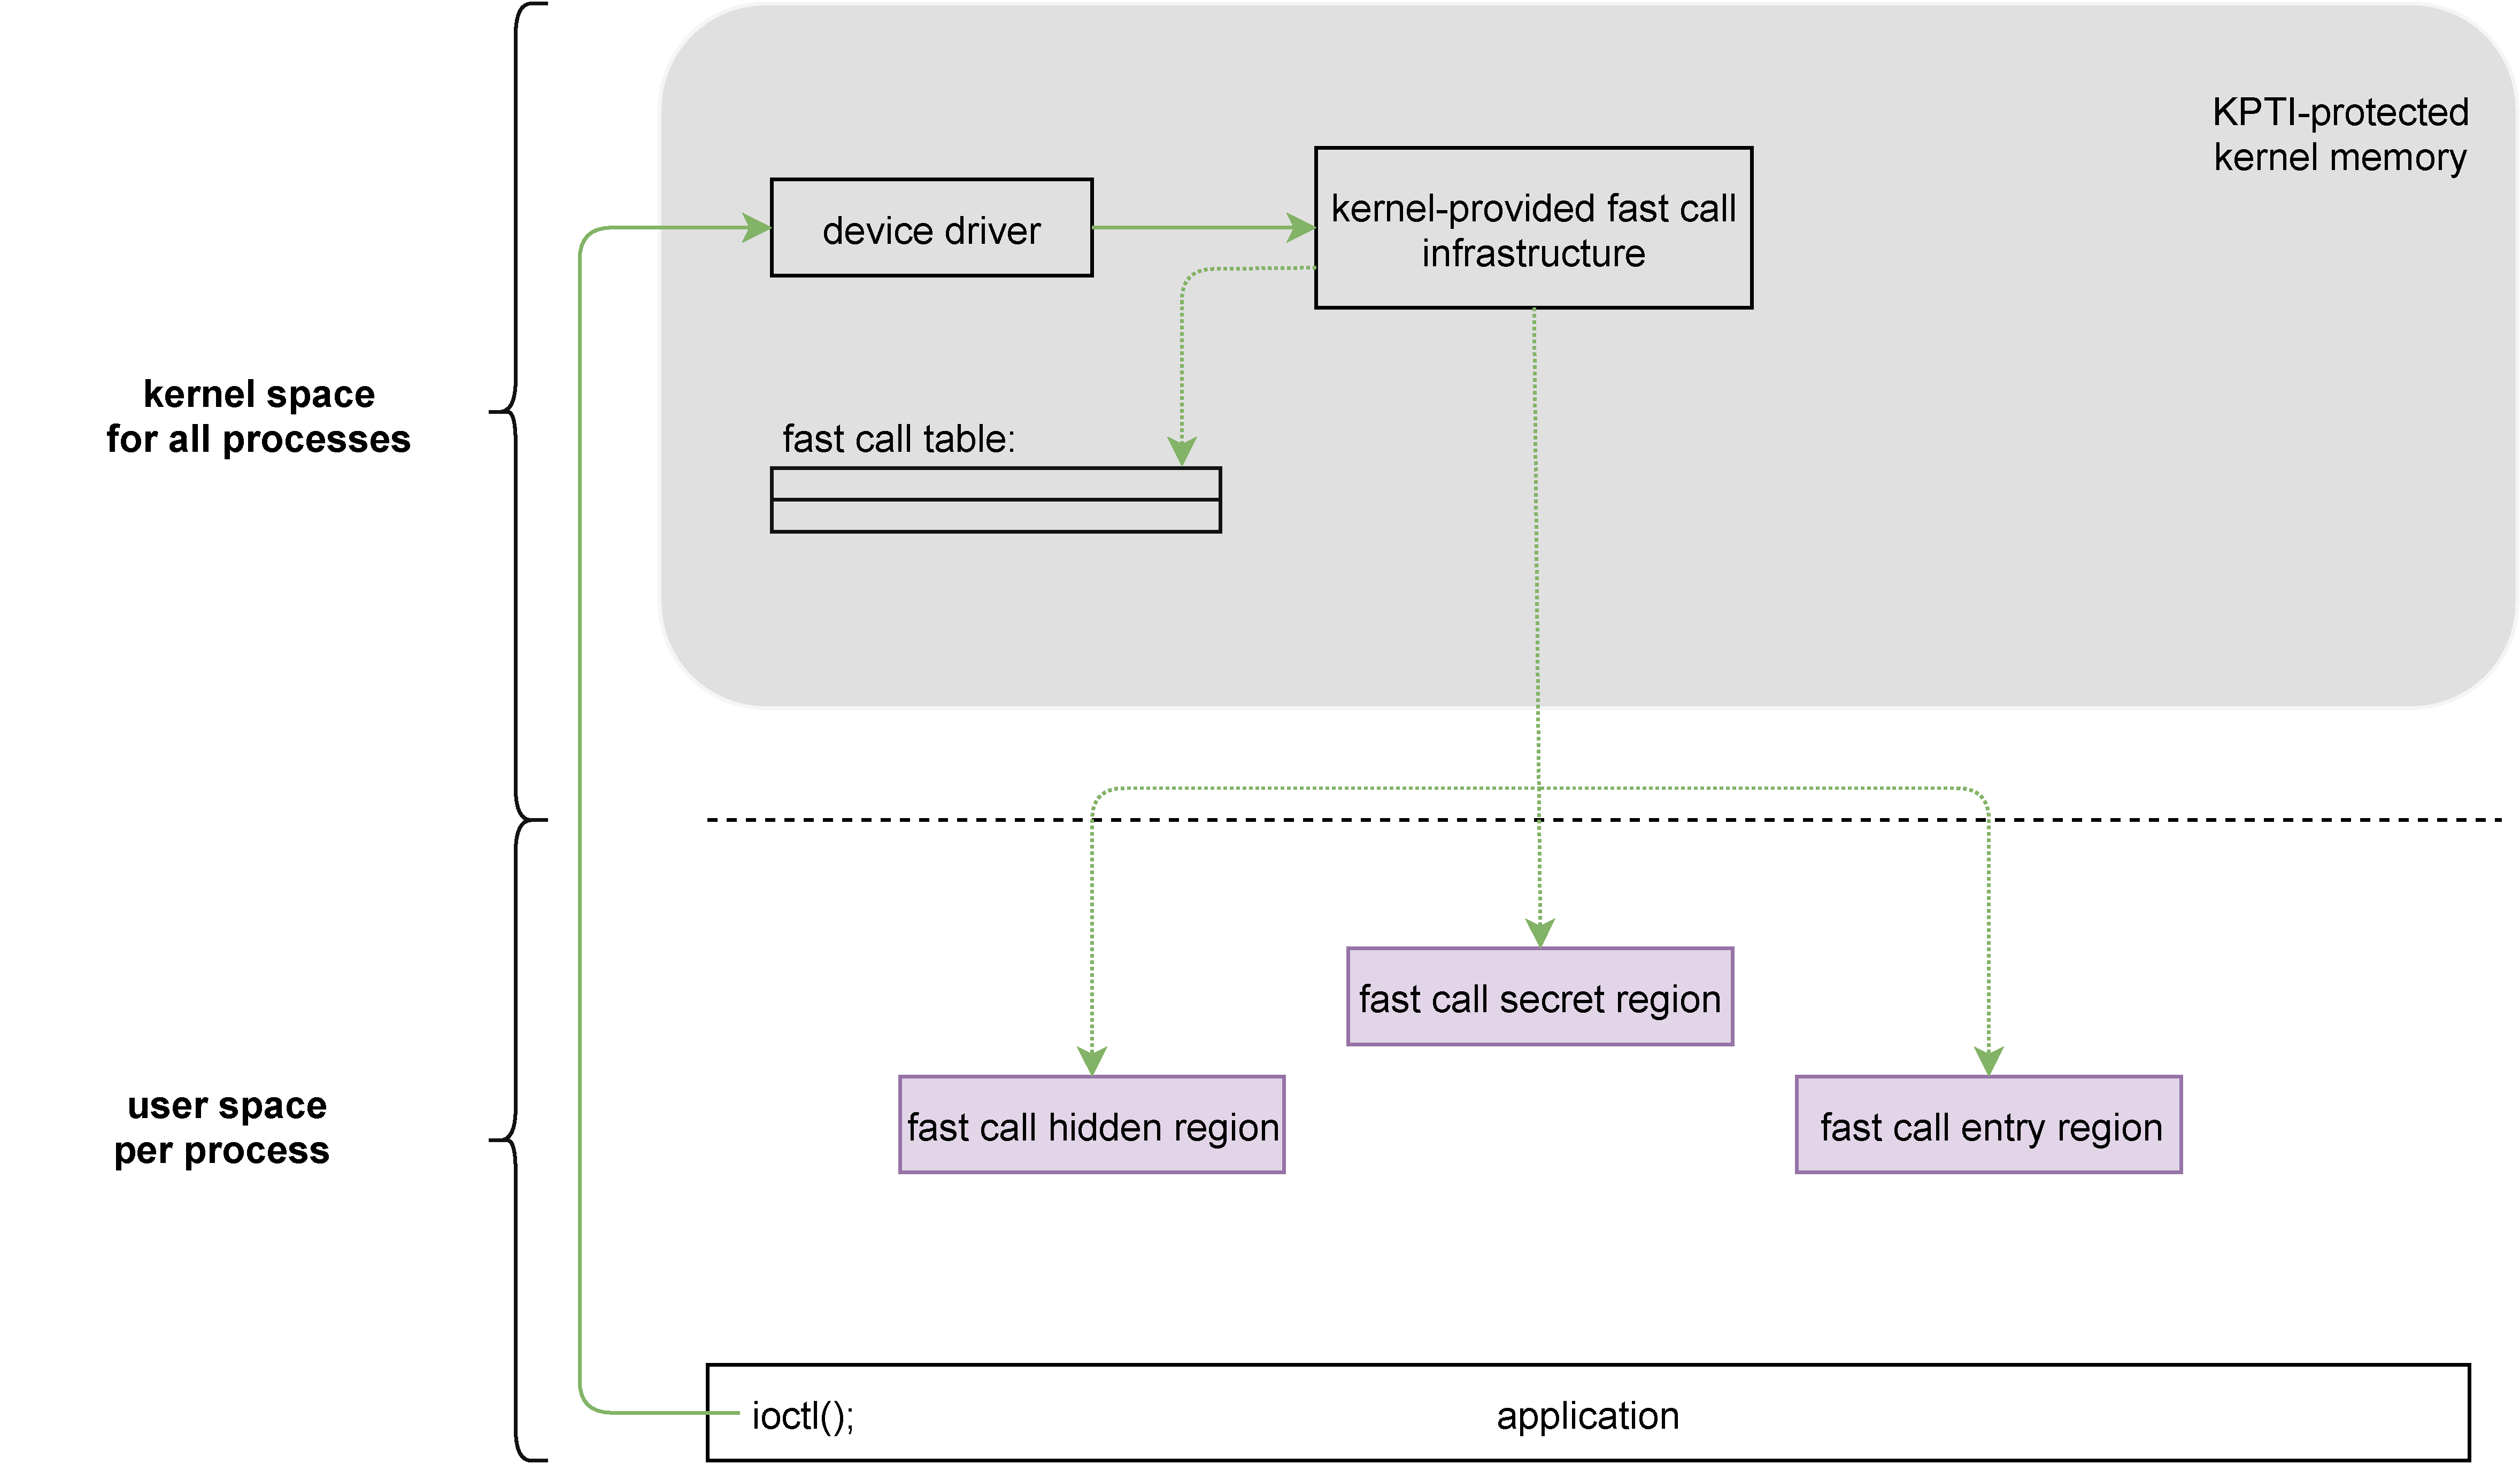
\includegraphics[width=0.8\textwidth]{images/registeration_process}
  \caption[Short description]{Fast Call Registration Process}
  \label{fig:registeration_process}
\end{figure}

Figure ~\ref{fig:registeration_process} shows the whole process of fast call registration:
\begin{enumerate}
  \item The process informs the device driver to register a fast call through the system call \emph{IOCTL}.
  \item The device driver:
    \begin{itemize}
      \item Copy the code for fast call entry and secret regions to page A and B separately.
        \begin{description}
          \item[Note:] The fast call mechanism supports creating a fast call entry region with a code length greater than 1 page. In this case, the code for the fast call entry region is copied to page array A.
        \end{description}
      \item Call the fast call registration function provided by the fast call infrastructure and pass pages A and B as parameters.
    \end{itemize}
  \item In the kernel-provided fast call infrastructure:
    \begin{itemize}
      \item Create the entry and secret regions in the process address space for the fast call and map pages A and B to entry and secret regions, respectively.
      \item Create fast call hidden regions for each device register and map each register to different hidden regions.
      \item Write each address of the fast call hidden regions into the page of the fast call secret region.
      \item Save the fast call information in the fast call table.
      \item Return the address of the fast call entry region
    \end{itemize}
  \item The driver returns the address of the fast call entry region to the process.
  \item The process calls the fast call through a function pointer to the address of the fast call entry region.
\end{enumerate}


\begin{figure}[tbp]
  \centering
  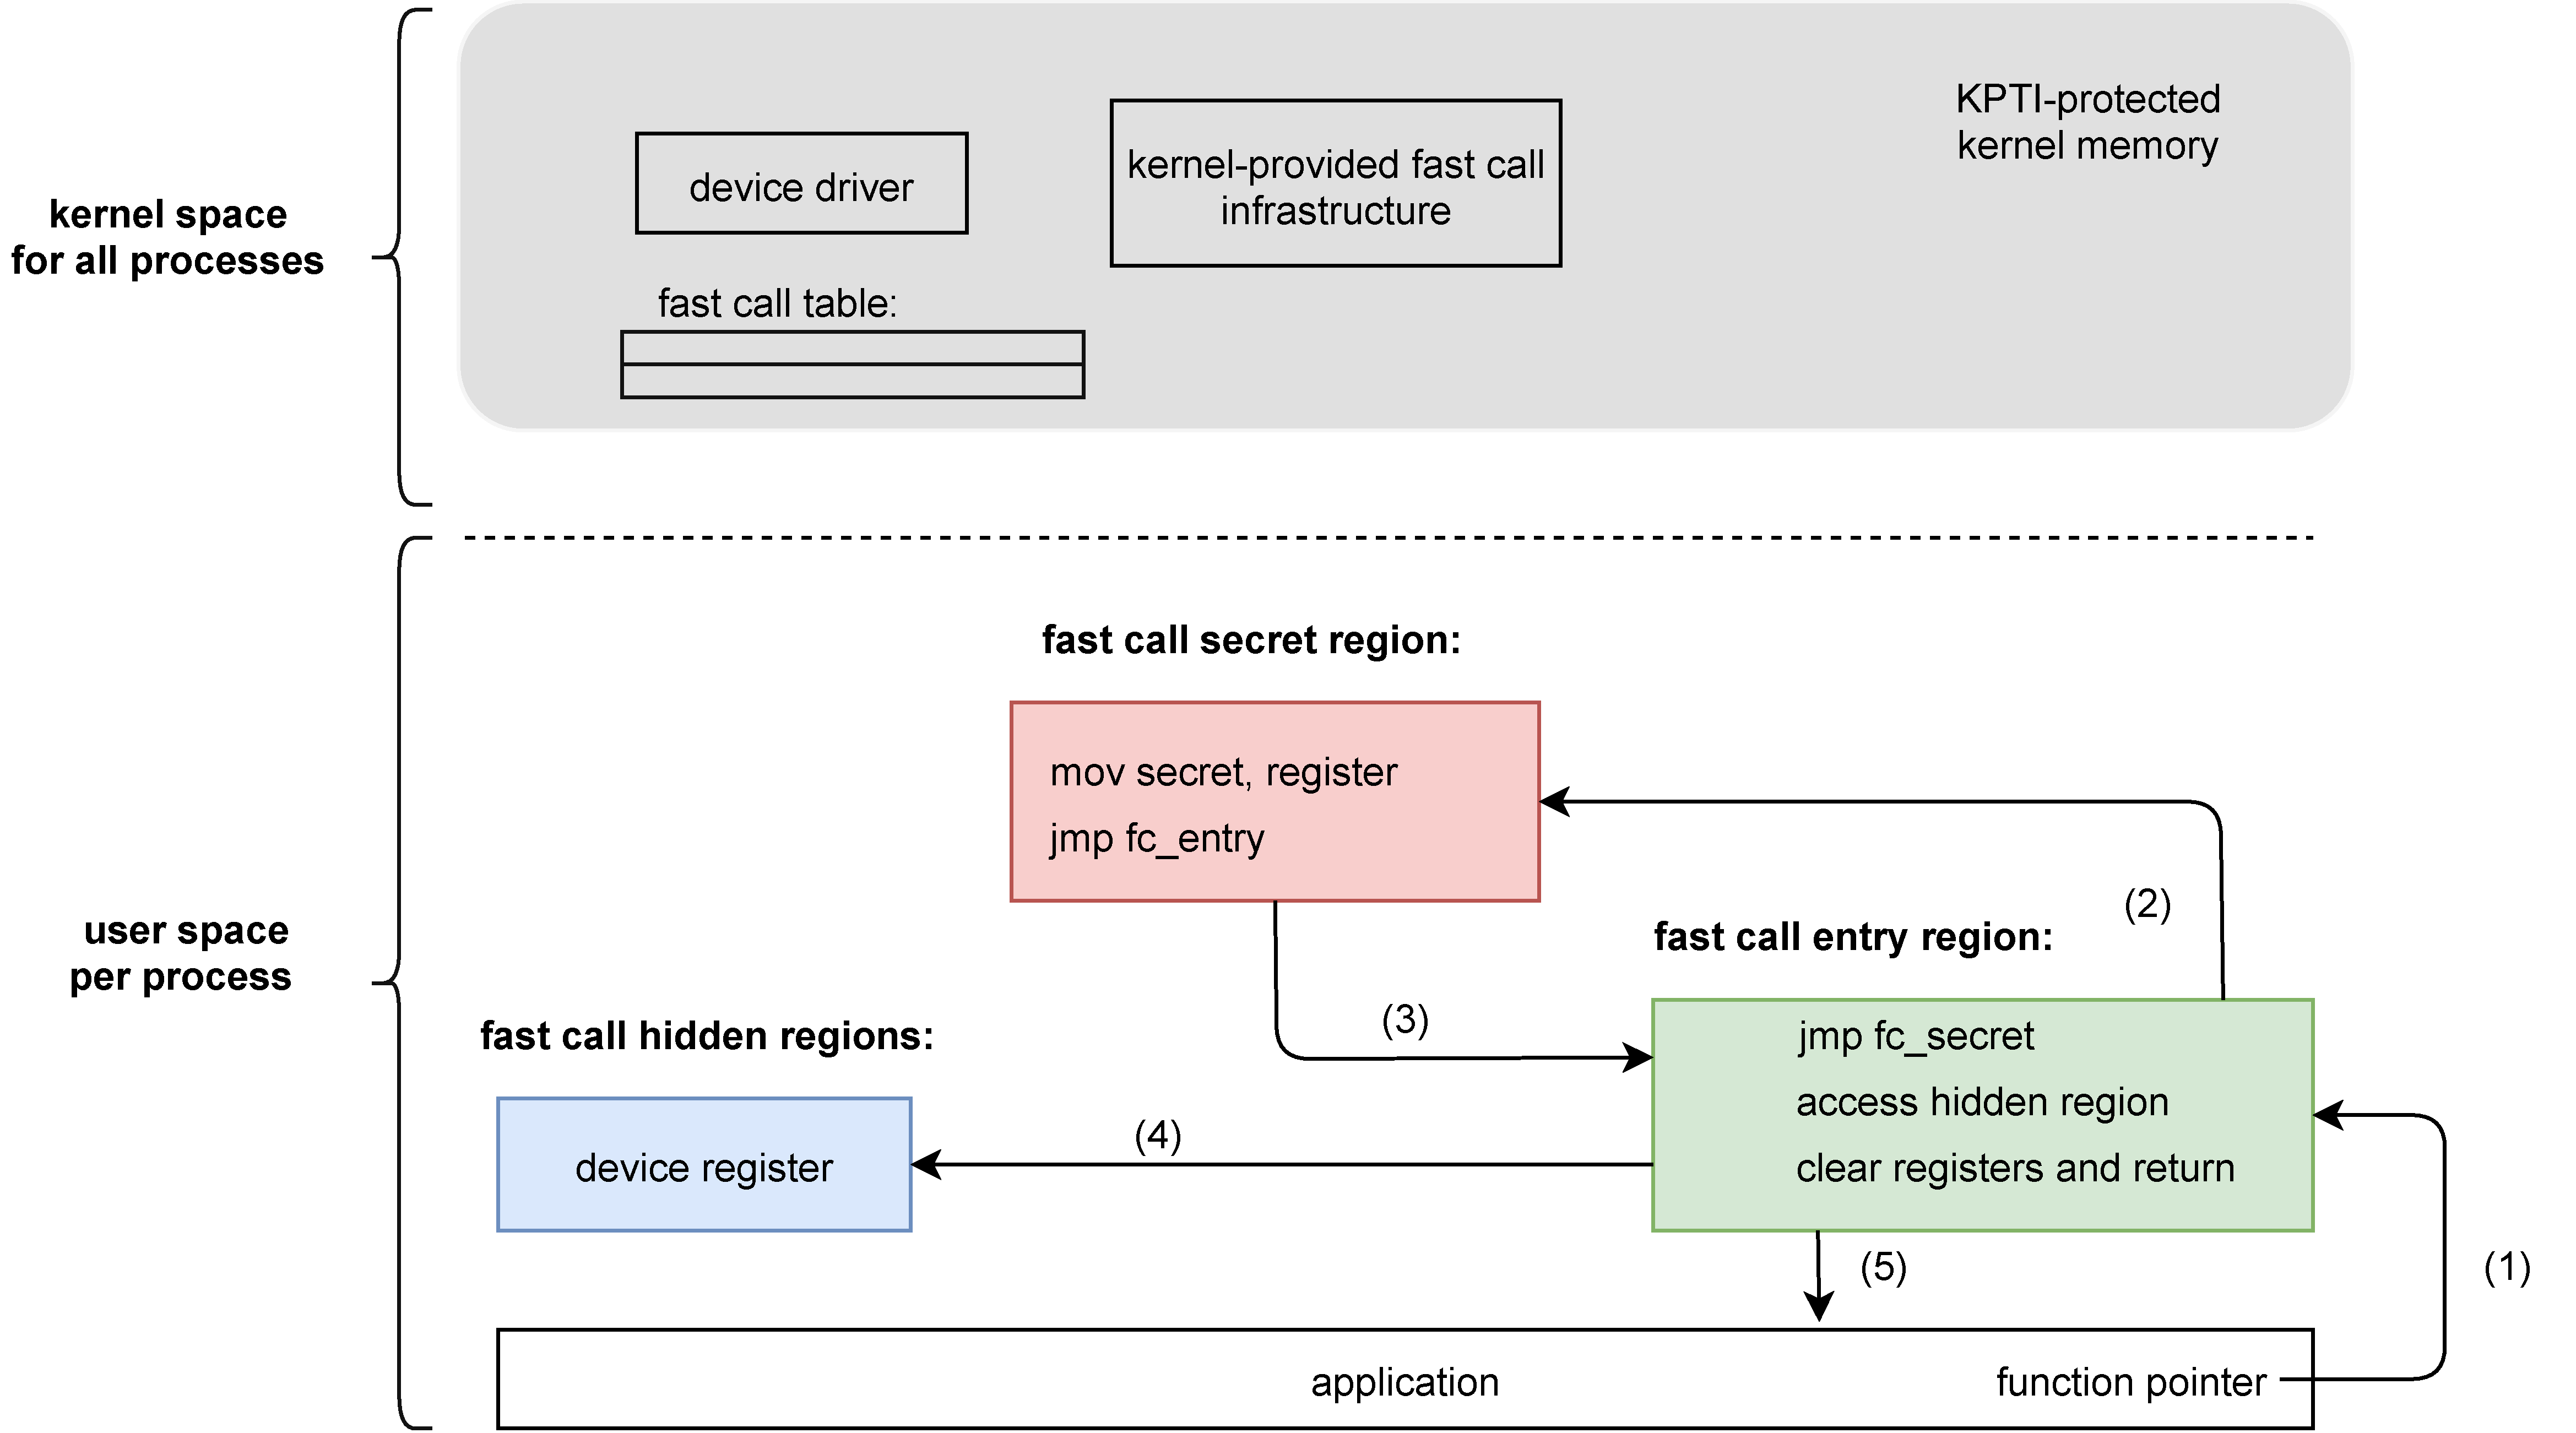
\includegraphics[width=0.8\textwidth]{images/fastcall_workflow}
  \caption[Short description]{Fast Call Work Flow}
  \label{fig:fastcall_workflow}
\end{figure}
\subsection{Fast call work flow}
Figure ~\ref{fig:fastcall_workflow} shows the fast call workflow on user space of a process:
\begin{enumerate}
  \item In the process:
    \begin{itemize}
      \item Define a function pointer to the fast call entry region.
      \item Use the defined function pointer to invoke the fast call.
    \end{itemize}
  \item The code on the fast call entry region uses a relative jump instruction \emph{jmp offset} to jump to the fast call secret region.
  \item In the fast call secret region:  
    \begin{itemize}
      \item Execute the instruction \emph{mov secret, register} to transfer the secret to a general-purpose register,  e.g., \emph{movq \$0x19016BC83000, \%rdx}.
        \begin{description}
          \item[Note:] The secret refers to the address of the fast call hidden region in the process address space.
        \end{description}
      \item Use relative jump instructions to return to the fast call entry region.
    \end{itemize}
  \item The fast call entry region continues to execute the code and access the fast call hidden region through the secret in the register.
  \begin{description}
    \item[Note:] The secret must always be in the register when the fast call is running. 
    Once the secret is taken out of the register and placed on the stack, 
    the secret  may be leaked since \emph{GDB} can view stack information.
  \end{description}
  \item The fast call entry region clears the secrets in the registers and returns the fast call execution result to the process.
\end{enumerate}

\section{Fast call table}
From the previous discussion, it is not difficult to see that two fast calls may run in different user spaces, and user spaces are isolated from each other. 
In this case, how should the fast call mechanism manage all fast calls? 

Fast call infrastructure chooses to use a table to manage registered fast calls. Each record in the table stands for a registered fast call.  
A record contains the address of the entry, secret, and hidden regions in a fast call.
Each record in the table is distinguished by the unique entry region address of the fast calls. 
This is possible because all fast call entry region addresses are randomized, i.e., every fast call 
has an individual entry region address as an identifier in the table. Thus, the in-kernel fast call 
infrastructure can find a specific fast call record in the table using the fast call entry region address as a key. 
The following few sections will introduce the fast call table’s internal structure and working principle.


\subsection{Placement of fast call table}
Suppose the fast call mechanism place a fast call table in each process address space to record 
the fast calls registered by each process. This is insecure and inefficient. Because the table is 
in the user space,  although we can randomize the address of the table, malicious users can still 
find the table by traversing the entire user space. Once the attacker finds the table,  
he can gain control of a device by accessing the device register mapped in a hidden region. 
On the other hand, one of the design goals of the fast call mechanism is to avoid the privilege 
transition as much as possible. Suppose the fast call table is placed in the user space. 
In that case, the fast call infrastructure would suffer two additional privilege transitions to 
add the fast call information into the corresponding table during the fast call registration process. 
Therefore, placing a table in each process user space is unwise.
The opposite of the user space is the kernel address space. One of the characteristics of the kernel address 
space is that all processes share the kernel address space. Therefore, it is possible to use a table in the 
kernel to record fast calls from different address spaces.
Specifically, placing the fast call table in the kernel space has the following advantages:
\begin{enumerate}
  \item The fast call mechanism only needs one table to record all fast calls, which means efficient space utilization.
  \item The fast call registration process can eliminate the performance loss caused by additional mode switching.
  \item The security of the fast call table is improved since the table is protected by the kernel.
\end{enumerate}

\begin{figure}[tbp]
  \centering
  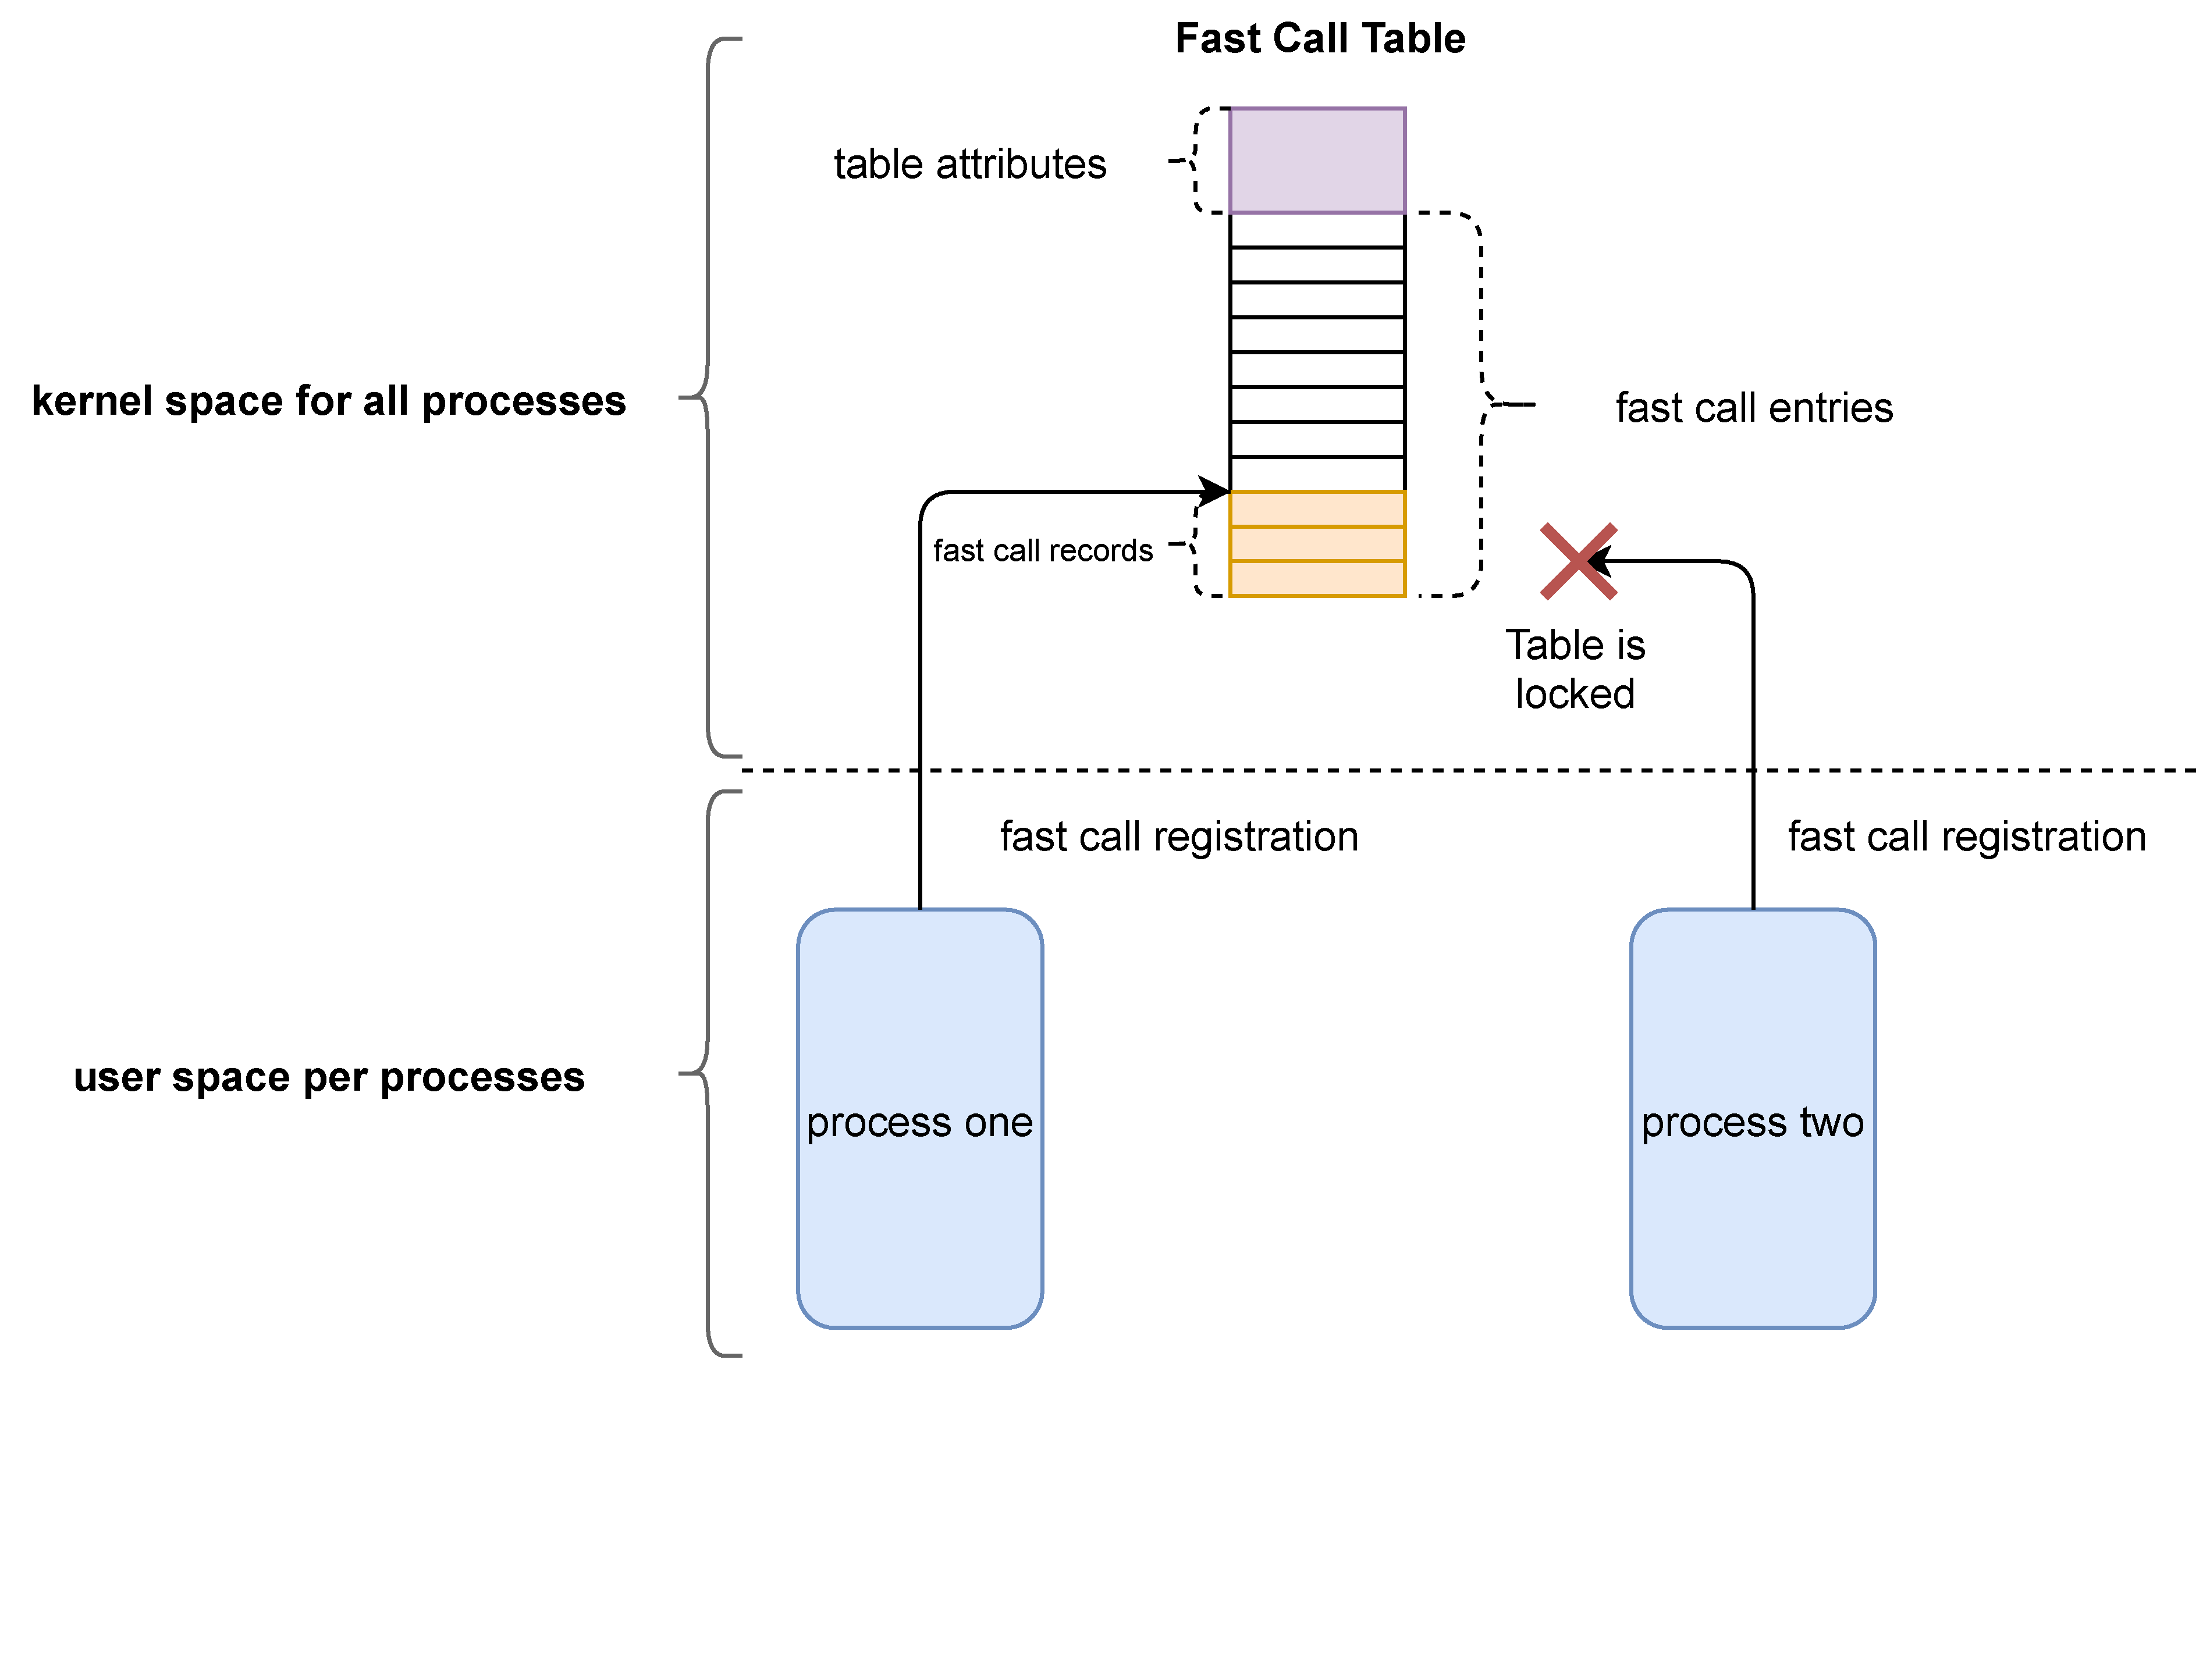
\includegraphics[width=0.8\textwidth]{images/fastcall_table}
  \caption[Fast Call Table]{Fast Call Table}
  \label{fig:fastcall_table}
\end{figure}

\subsection{The structure of the fast call table}
As shown in Figure ~\ref{fig:fastcall_table},the fast call table mainly comprises two parts, 
the entries, and the table attributes. 
Each entry is used to record a fast call's information, 
such as each component's address in a fast call and the number of 
hidden areas supported by the fast call. Fast call records represent the registered fast calls. Table attributes mainly 
contain two variables. The first variable \emph{entries\_size} 
records the number of fast calls in the table. Another variable is a 
\emph{mutex} that prevents two processes from accessing the table at the same time.


\subsection{Allocation and deallocation}
The memory resources in the kernel are very scarce. 
Therefore, the fast call mechanism chooses to allocate memory dynamically for the fast calling table. 
Whenever a process registers for a fast call, the fast call mechanism 
first checks whether the table has been allocated and initialized. If not, the fast call mechanism will 
first allocate memory for the table and then complete the fast call registration process.
Similarly, the fast call mechanism checks the number of fast call records in the table during the fast 
call deregistration process. If the number of fast call records in the table is 0, the table's memory will be released.
All in all, by dynamically allocating and releasing the table's memory when registering and unregistering a 
fast call, the fast call mechanism realizes the efficient use of kernel memory and avoids possible memory leaks. 

\subsection{Distinguish fast calls}
The fast call table uses the address of the fast call entry region to distinguish 
fast calls from each other because each fast call only has one entry region, and each 
entry region's address is unique.  When the in-kernel fast call infrastructure creates 
a fast call, it first randomizes the fast call entry region's address. As a result, 
fast calls in the same and different process address space have a unique fast call entry 
region address. Thus, the fast call infrastructure can use this address as a key to finding the corresponding record in the table.


\subsection{Fast call record}

Speaking of the records in the table, as shown in the figure, it contains information about 
a fast call.  Remember that we mentioned in the design chapter that 
a fast call includes:
\begin{itemize}
  \item The entry region.
  \item The secret region.
  \item The hidden regions.
\end{itemize}
Because a device may have multiple control registers, 
the fast call mechanism supports the creation of numerous 
hidden regions for a fast call to map the device control registers to different locations in 
the user address space. Based on the above considerations, each record includes the addresses of 
the entry region, the secret region, and multiple hidden regions. 
In a record, the number ratio of the entry region to the secret region 
to the hidden region is 1:1: n.
\begin{figure}[tbp]
  \centering
  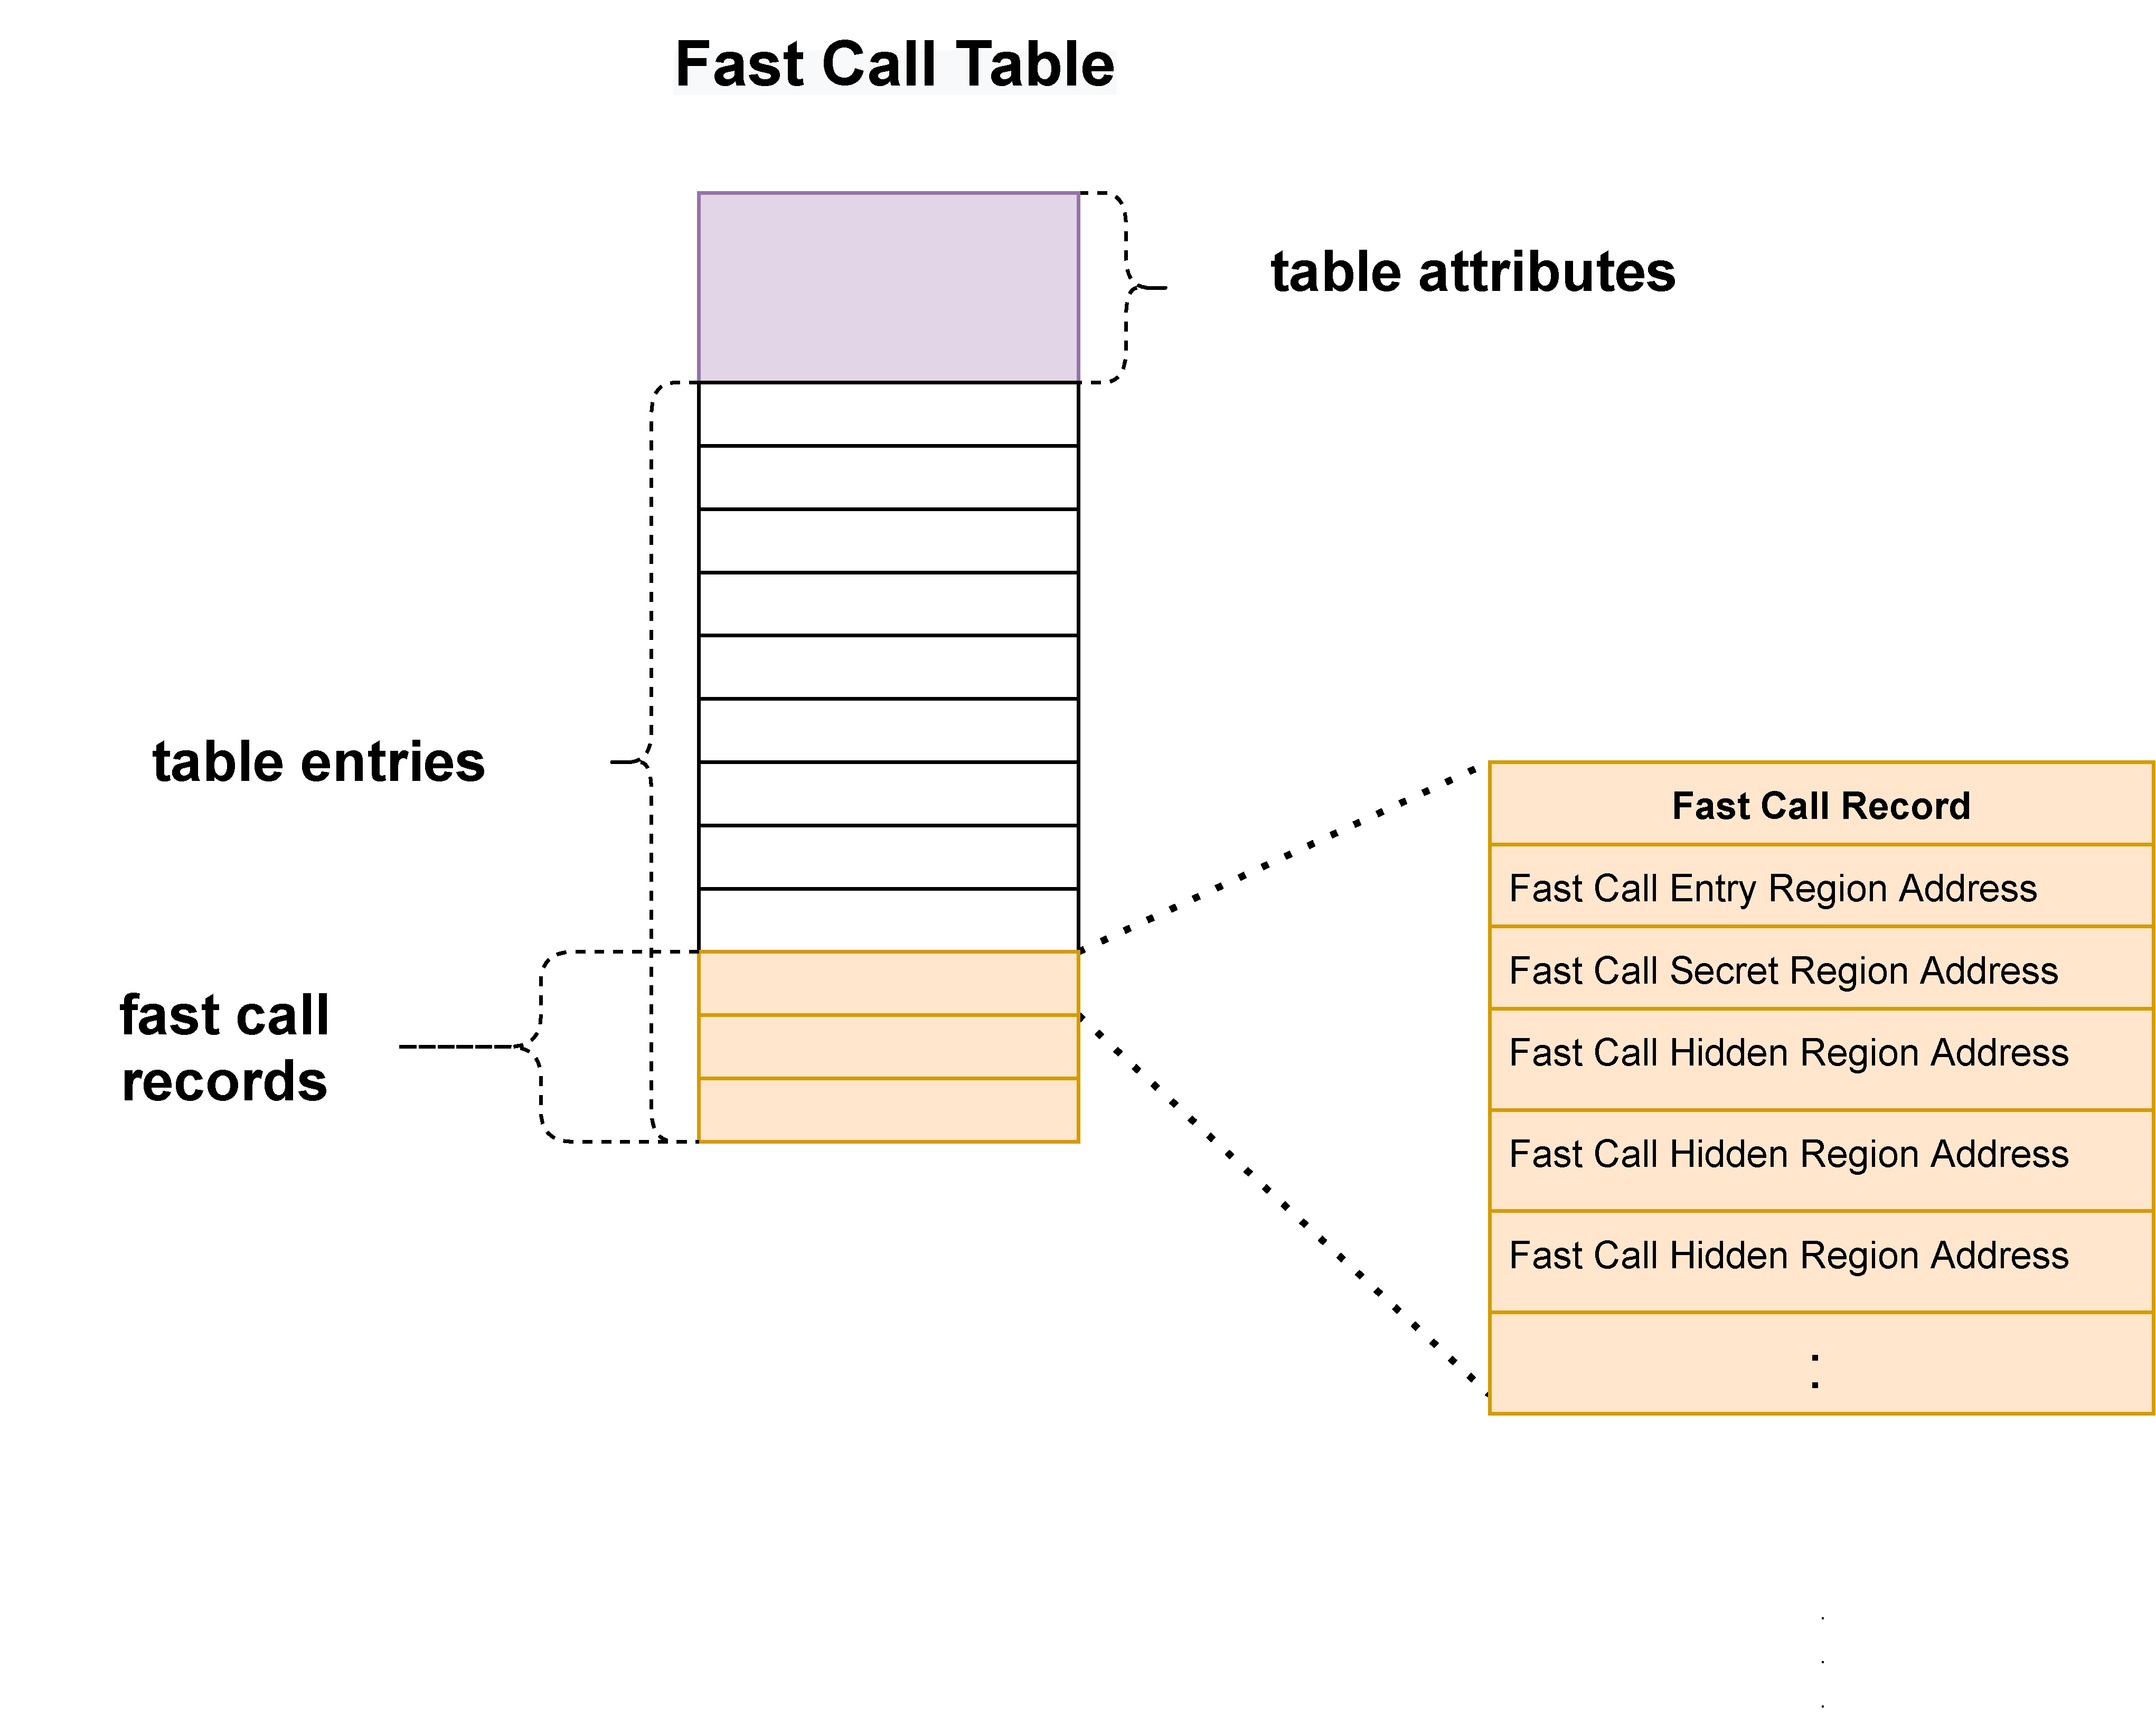
\includegraphics[width=0.8\textwidth]{images/Fast_Call entries}
  \caption[Fast Call Entry]{Fast Call Entry}
  \label{fig:Fast_Call_entries}
\end{figure}
Generally speaking, a fast call record is created when the 
fast call is registered and deleted when the fast call deregistration 
function is called.

What if a process registered with fast calls does 
not call the deregistration function and terminates directly? 
Specifically, suppose that a process suddenly terminates after 
registering multiple fast calls. The unregister function is not 
called to delete the corresponding records in the fast call table. 
In this case, multiple zombie records will appear in the table. 
Therefore, the table's memory can no longer be dynamically released, 
which means a memory leak occurs in the table.

The fast call mechanism solves this problem with the help 
of the data structure called \emph{mm\_struct}.  The data structure \emph{mm\_struct}
represents the process address space descriptor\cite{10.5555/983550} in the kernel, which contains a list of virtual memory area.
 Most resources, including the process address space descriptor, 
 are tracked through a reference counter in the Linux kernel.  
 When the reference counter is reduced to zero, the kernel invokes the 
 \emph{deconstructor} to recycle the resource since no one uses the resource anymore.  
 Specifically, a process address space descriptor is released when all threads 
 running on the address space are terminated. 

The fast call mechanism exploits this resource management mechanism 
in the kernel to delete zombie records in the fast call table. 
In the address space descriptor's \emph{deconstructor}, the fast call mechanism 
checks whether the address space contains virtual memory areas belonging 
to fast calls. If there is, it deletes the corresponding fast 
call records in the fast call table.


\section{Fast call mapping}
This section focuses on mapping the three components of a fast call in the process address space. 
In particular, we introduce how to prevent others from manipulating the mapping belonging to fast 
calls and other issues related to the fast call mapping in the process address space.

\subsection{Prohibiting others from operating the mapping belonged to fast calls}
Remember that we introduced in Chapter \emph{Design} 
that a fast call is roughly composed of three parts: 
entry, secret, and hidden regions. From the kernel's perspective, 
these three fast call components are just three virtual memory 
areas(\emph{VMA})\cite{10.5555/983550} represented by \emph{vm\_area\_struct} in a process address space and 
tracked by a list in process address space descriptor\cite{10.5555/983550}.

Therefore, the kernel (or user-level process) can modify these three virtual memory areas 
through specific functions (or system calls). 
For example, change the location (address) of the virtual memory areas in the process address space, 
unmap the virtual memory areas, or swap pages mapped in a virtual memory area to disk. The consequences
 are unimaginable if a process or the kernel can manipulate the memory mapping related to a fast call. 
 Suppose the kernel can unmap a fast 
call's secret region without authorization of the fast call mechanism. 
In this case, the fast call entry region cannot communicate with the hidden regions anymore 
since it can not retrieve the secret region's address from the secret region anymore. 
More seriously, this will cause the fast call infrastructure to crash during the fast call 
deregistration because it cannot unmap the secret region correctly. In addition, the secrets 
stored in the secret region would be invalid if the hidden regions are move to other locations by the kernel.


As Kernel design and implementation explained:\textquote{
The field \emph{VMA} operations in the virtual memory area descriptor points 
to the table of operations associated with a given virtual 
memory area, which the kernel can invoke to manipulate the \emph{VMA}. 
The virtual memory area descriptor acts as a generic object for any type of memory area, 
and the operations table describes the specific methods that can operate 
on this particular instance of the object.} Specifically, when the kernel wants to change 
the address of a \emph{VMA}, e.g., unmap it, the kernel calls the method in the table to complete 
those operations. Therefore, when a process registers a fast call through the API provided 
by the in-kernel fast call infrastructure, the infrastructure customizes the following three 
specific methods in the table associated with the \emph{VMAs} that belonged to this fast call to avoid 
those \emph{VMAs} from been manipulated without the authority of the fast call infrastructure.
\begin{lstlisting}[style=CStyle]
  /*
   * fastcall_mremap - prohibit remap the fast call entry region, secret region, and hidden regions
   */
 static int fastcall_mremap(const struct vm_special_mapping *sm, struct vm_area_struct *new_VMA)
 {
   /* Invalid argument */
   return -EINVAL;
 }

 /*
  * fastcall_may_unmap - prohibit unmap the fast call entry region, secret region, and hidden regions
  */
static int fastcall_may_unmap(const struct vm_special_mapping *sm,
			      struct vm_area_struct *VMA)
{
	/* Permission denied */
	return -EACCES;
}

/*
 * fast call_fault - every fault to this \emph{VMA} is invalid
 */
static vm_fault_t fastcall_fault(const struct vm_special_mapping *sm,
				 struct vm_area_struct *VMA,
				 struct vm_fault *vmf)
{

	return VM_FAULT_SIGBUS;
}
\end{lstlisting}

The function \emph{fastcall\_mremap} prohibits the kernel 
(or user-level process) from modifying the location of any virtual 
memory area related to fast calls. Once the \emph{VMAs} are mapped to a 
process address space, those \emph{VMAs}  cannot 
be changed unless the process deregisters the fast call. The function 
\emph{fastcall\_may\_unmap} is similar to \emph{fastcall\_mremap}. This function 
prevents others from unmapping \emph{VMAs} belonging to fast 
calls without the permission of the in-kernel fast call infrastructure. 
Typically, The \emph{VMAs}  belonging to a 
fast call will not generate a page fault since the pages mapped in the 
fast call's \emph{VMA} are kept in memory. Just in case, we set up the page fault 
handling function to return an error. Do not worry. We will explain in 
the following paragraphs why pages mapped to \emph{VMAs} belonging to fast calls 
are not swapped out.


\subsection{\emph{VMA} flags of fast call components}
As mentioned in Chapter 3, the entry region should be readable and executable in a fast call. 
The secret region should be only executable. The hidden region should be readable and writable. 
How to achieve this design decision?

The solution is straightforward. When the fast call mechanism initializes 
\emph{VMAs} for the components in a fast call, it will add flowing flags for 
each \emph{VMA}. These flags determine the access rights of a \emph{VMAs}.

\begin{lstlisting}[style=CStyle]
  /* Flags for entry region */
  VM_READ| VM_MAYREAD|VM_EXEC |VM_MAYEXEC

  /* Flags for secret region */
  VM_EXEC | VM_MAYEXEC

  /* Flags for hidden region */
  VM_READ | VM_MAYREAD | VM_MAYWRITE | VM_WRITEVMA
\end{lstlisting}


In addition, to ensure that all pages mapped to fast calls' \emph{VMAs} 
are not swapped out, the fast call mechanism also adds the flag \emph{VM\_LOCKED} 
to each \emph{VMA}. The advantage of this is to improve the performance of 
fast calls because the page fault is very time-consuming.

Finally, the flag \emph{VM\_DONTCOPY} is added to all the fast calls' \emph{VMAs} to prevent 
them from copying from their process address space to a new process address space 
under the fork system call. The reason is that the fast call table requires that each 
fast call has a unique entry region address to distinguish the fast call records in 
the table. For example, the fast call deregistration function uses the fast call entry 
region's address as the key to looking for the corresponding record in the table and then 
unmaps the fast call from the corresponding address space and deletes the entry in the table. 
Assume that processes A and B have the fast call with the same entry region address in their 
address space, respectively. When A unregisters the fast call in its address space, 
the fast call deregistration function deletes the corresponding record in the table 
before returning. This has led to B's inability to unregister its fast call because 
the fast call deregistration function cannot find the corresponding record in the table.


\subsection{Is only executable memory region really possible?}

Remember that we set the fast call secret region's VMA with the flag \emph{VM\_EXEC} 
since we expect the \emph{VMA} to be only executable. But it is not the case. The \emph{VMA} 
with flag \emph{VM\_EXEC} is readable and executable. The reason is that the current X86 architecture does not support none readable memory region, in other words, the only executable region.  
Internally, according to the page table, the \emph{MMU} manages the mapping between the virtual address and the physical address in page granularity. In addition, the MMU also handles the memory 
protection based on the permission bit on the page table entry. For example, the \emph{MMU} sends a segmentation fault to a process if the process tries to write something to an only readable memory area. 
Each page table entry on x86 architecture has three important permission bits:

\begin{itemize}
  \item \emph{PTE\_U}:  a user-level process can not access the page if \emph{PTE\_U} = 0. 
  \item \emph{PTE\_R}:  \emph{PTE\_R} = 0 stands  for read-only, \emph{PTE\_R} = 1 stands for read-write.
  \item \emph{PTE\_XD}: \emph{PTE\_XD}= 0 stands for executable, \emph{PTE\_XD}= 1 stands for non-executable.
\end{itemize}

When the kernel creates a \emph{VMA} with certain flags such as \emph{VM\_EXEC} and \emph{VM\_READ} in a process address space,  it also sets the permission bits on certain page 
table entries corresponding to the pages mapped into the \emph{VMA} so that the \emph{MMU} can manage the memory access permission correctly. In our case, we assign the secret region's \emph{VMA} the flag 
\emph{VM\_EXEC}. Since x86 architecture dose does not have a special permission bit for none readable permission, the kernel only sets the \emph{PTE\_R = 0} and \emph{PTE\_XD = 0}, which means the pages mapped to the secret region are readable and executable.  
Therefore, it is not possible to have an only executable memory region on x86 architecture.


\section{Fast call entry/hidden region randomization}


Randomizing the location of the fast call entry and hidden region is essential. 
The first reason comes from security considerations. 
When the kernel allocates a \emph{VMA} in a process address space, it starts from a 
certain lower address in the address space to find a location suitable for the 
size of the \emph{VMA}. Therefore, two \emph{VMAs}  allocated one after the other may be in adjacent 
positions. Assume a fast call contains one entry, one secret, and one hidden region. 
When the in-kernel fast call infrastructure creates the fast call, it allocates three 
virtual memory areas in the current address space. If the location of the entry and hidden 
regions are not randomized, three areas will likely be placed in the address space adjacently. 
Since the address of the fast call entry region is returned to the user and three regions are 
adjacent, a malicious user can easily infer the location of the hidden region. The second reason 
is that the fast call table requires the address of the entry region in each fast call to be unique. 
The fast call table uses the entry region address in each fast call to distinguish different fast calls.


Randomizing the location of the fast call entry and hidden region is essential. 
The first reason comes from security considerations. 
When the kernel allocates a \emph{VMA} in a process address space,  it searches 
for a location suitable for the size of the \emph{VMA} in the address space from 
bottom to top. The address to start the search is determined by the variable 
\emph{low\_limit}, as shown in the Figure ~\ref{fig:mmap_search_methods}. Therefore, two \emph{VMAs} 
allocated one after the 
other may be in adjacent positions. Assume a fast call contains one entry, one secret, 
and one hidden region. When the in-kernel fast call infrastructure creates the fast call, 
it allocates three virtual memory areas in the current address space. If the location of 
the entry and hidden regions are not randomized, three areas would likely be placed in the 
address space adjacently. Since the address of the fast call entry region is returned to the 
user and three regions are adjacent, a malicious user can easily infer the location of the 
hidden region. In addition, the fast call table requires the address of the entry region in 
each fast call to be unique. The fast call table uses the entry region address in each fast 
call to distinguish different fast calls. Thus, the location of entry and secret regions in a 
fast call must be randomized.
\subsection{Randomization method}
\begin{figure}[tbp]
  \centering
  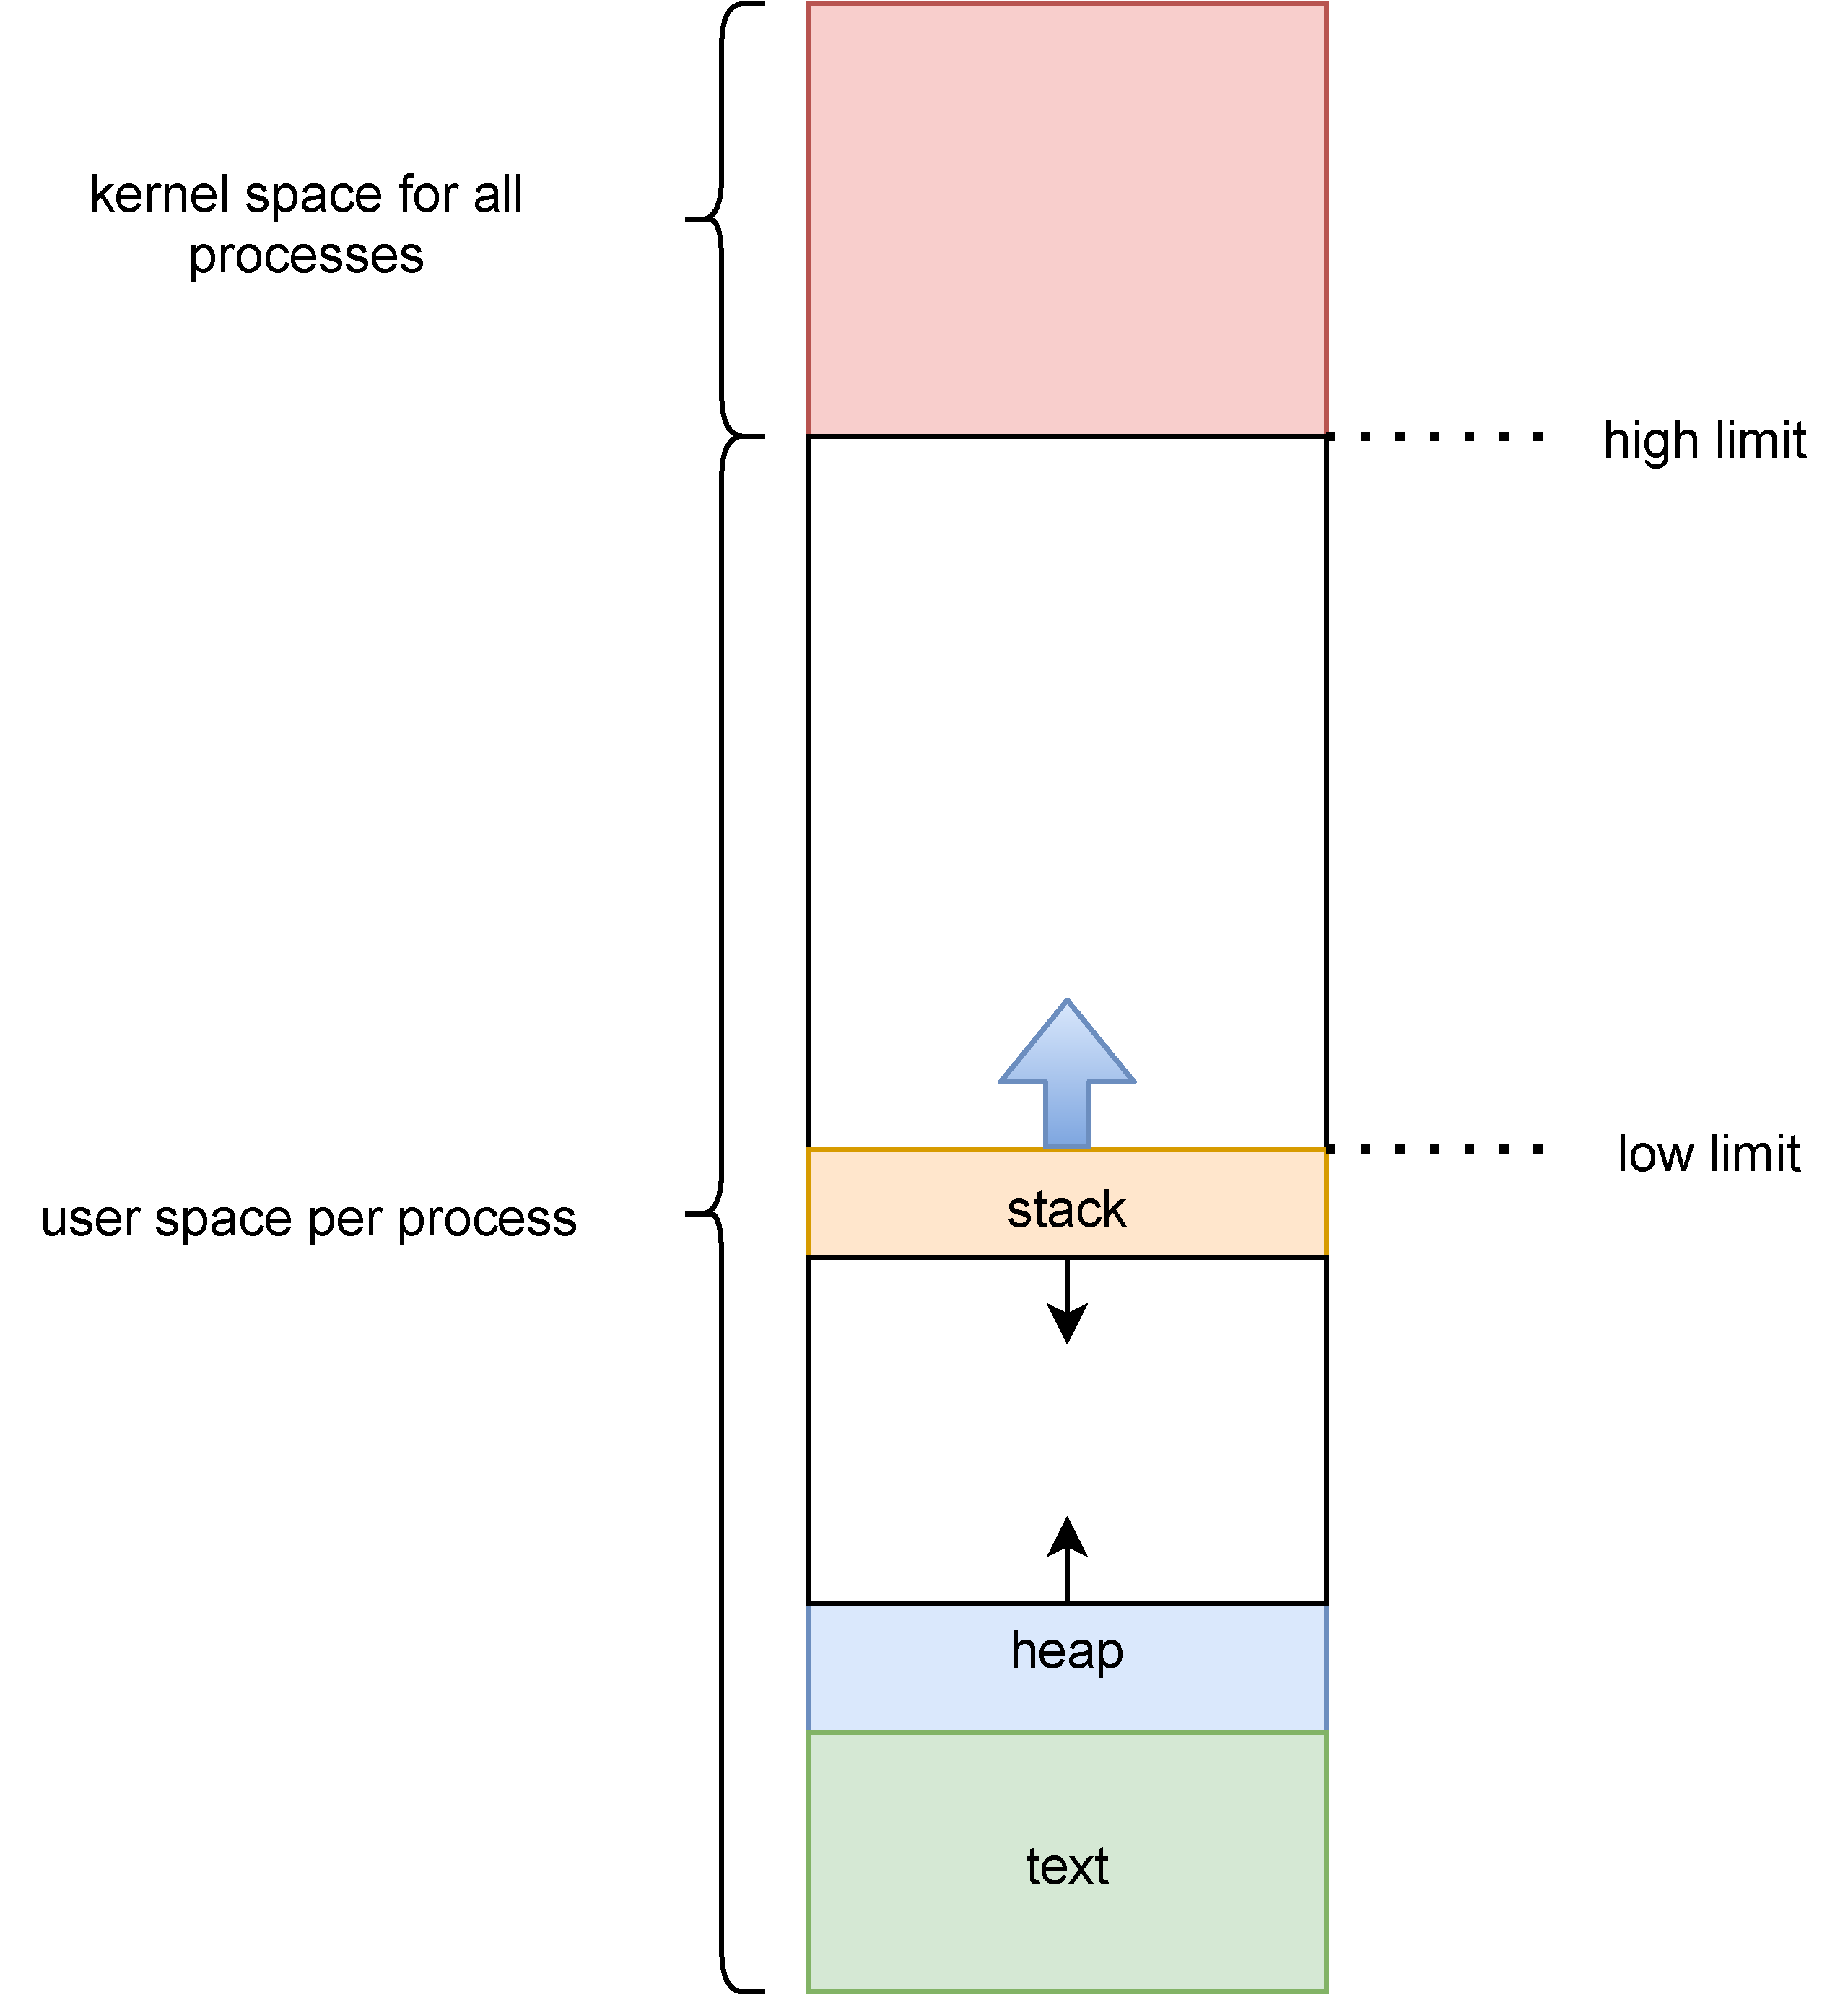
\includegraphics[width=0.8\textwidth]{images/mmap_search_methods}
  \caption[Short description]{Mmap() workflow}
  \label{fig:mmap_search_methods}
\end{figure}



First, let us study the process of creating a \emph{VMA} by the kernel. 
The kernel creates a \emph{VMA} mainly in two steps. In the first step, 
as shown in Figure ~\ref{fig:mmap_search_methods}, the kernel calls 
a function searching an area suitable for the size of the \emph{VMA}  in the corresponding 
address space and returns the starting address \emph{A} of the area. In the second step, 
The kernel creates a \emph{VMA} and add it to the address \emph{A} in the address space.  
Note that in the first step, the search 
function always starts searching from the address \emph{low\_limit}.
Based on the above workflow, the fast call mechanism leverage the randomization 
of the address \emph{low\_limit} to randomize the fast calls' \emph{VMA} location. Precisely,  
when the fast call infrastructure allocates \emph{VMAs} in the process address space for 
the entry and hidden regions, it generates a 64-bit random number and 
reserve the lower 46  bits of the number serve as the starting address for 
the kernel to search for a suitable area for this \emph{VMA}. In this way, the search 
function starts from a different location each time. Therefore,  the location 
that the kernel found for the \emph{VMA} is randomized too. 


\section{Secret region and secret}

This section focuses on the fast call's secret region and 
secrets on it. We will introduce how the secret is placed on the secret region, how the code on 
the entry region retrieves the secret from the secret region, 
and how the entry region guarantees that the secret obtained will not be leaked.

\subsection{Secrets placement issue on secret region}
The previous section analyzed the reasons and methods of address randomization 
for the fast call hidden region. Note that secrets on the secret region refer 
to the addresses of the hidden regions. In addition, the address randomization 
is performed at runtime. Therefore, the fast call mechanism cannot write the 
secrets at compile time to the page that will be later mapped to the secret region.

\begin{figure}[tbp]
  \centering
  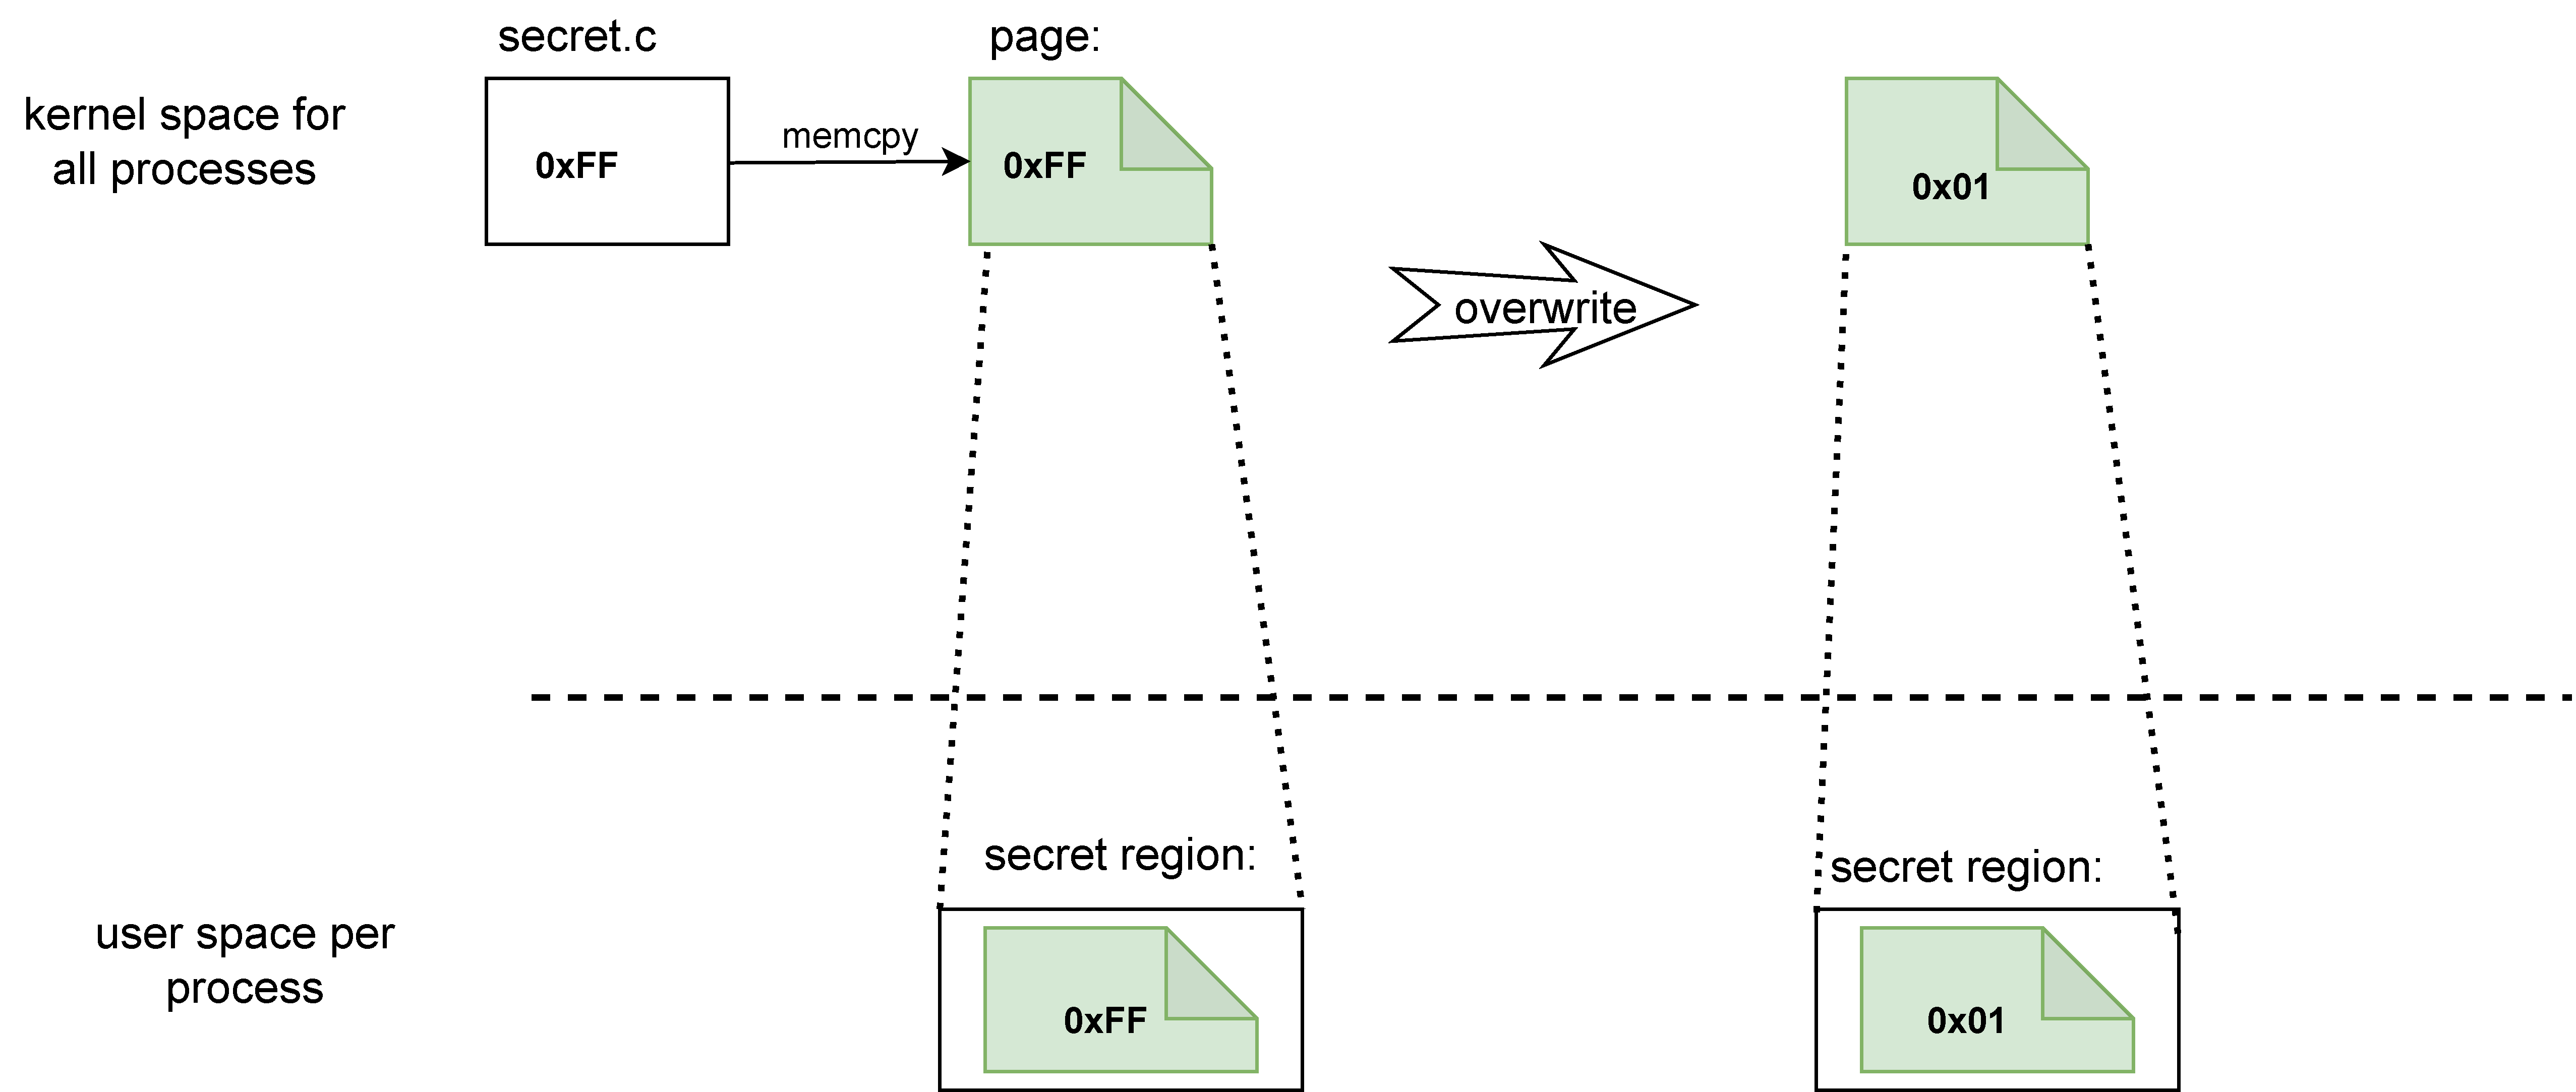
\includegraphics[width=0.8\textwidth]{images/secret_pages}
  \caption[Short description]{Secrets on the page mapped to the secret region}
  \label{fig:secret_pages}
\end{figure}

Figure \ref{fig:secret_pages} shows the workflow of fast call mechanism for writing secrets into the secret region. 
During the fast call registration process,
the diver copies the file "secret" to a page and passes the page as a parameter to
 the fast call infrastructure. The fast call infrastructure first creates an entry 
 region and secret region for the fast call and maps the page to the secret region. 
 Note that what is stored on the page is still dummy value \emph{0xFF} for now. The fast call 
 infrastructure then creates a hidden region. Now that the fast call infrastructure 
 already knows the hidden region address, it overwrites the dummy value with the hidden 
 region address \emph{0x01} on the page by mapping the page to the kernel space. In this way, the fast call mechanism 
 successfully writes the secret into the secret region.


 \subsection{Secret movement between entry and secret region}
 However, it is not enough to only place secrets
 (addresses of the fast call hidden regions) on the fast call secret region. 
 Because the secret region is only executable, the entry region's code cannot 
 get the secrets out by reading the secret region's memory(using a pointer).
To achieve the goal of extracting the secret to the fast call entry region, 
  we must use \emph{mov}, \emph{jmp} instructions, and labels in assembly.

 \begin{figure}[tbp]
   \centering
   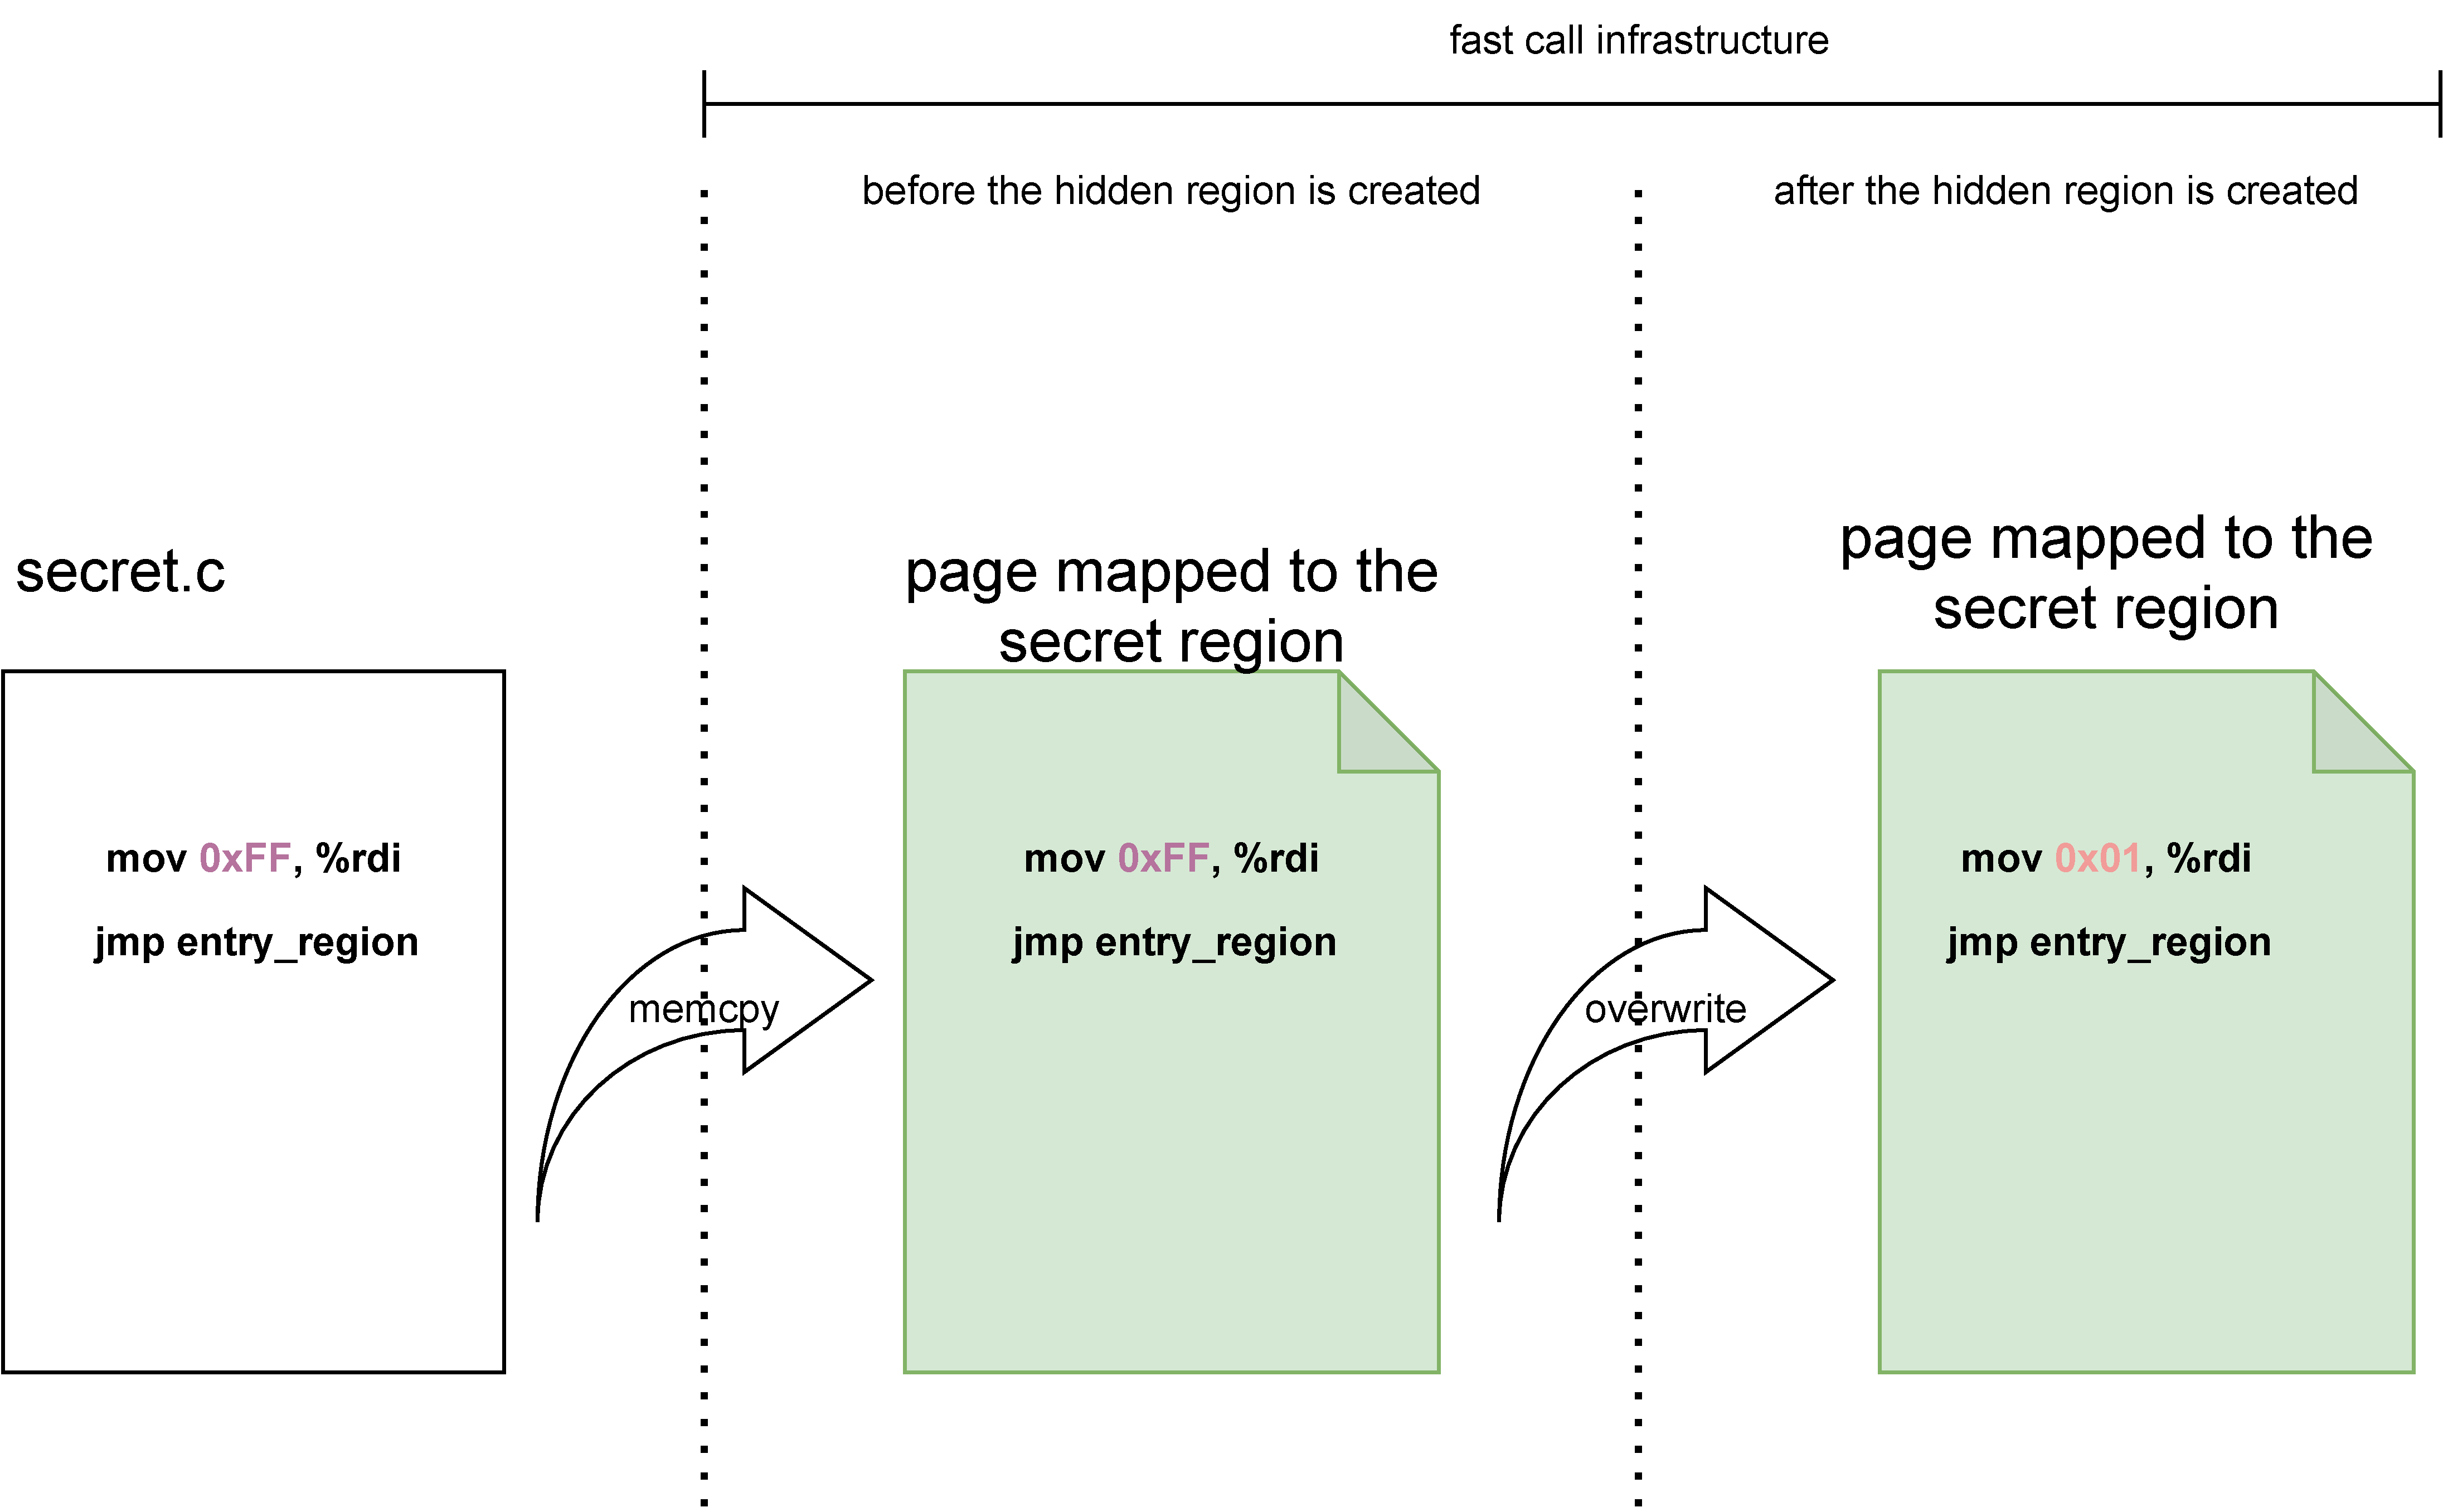
\includegraphics[width=0.8\textwidth]{images/secret_pages_2}
   \caption[Short description]{Secrets on the page mapped to the secret region, version 2}
    \label{fig:secret_pages_2}
 \end{figure}
  
 In the real implementation shown in Figure \ref{fig:secret_pages_2}, 
 we place multiple \emph{mov} instructions on the page,
 and a \emph{jmp} instruction follows each \emph{mov} instruction. Note that the page is mapped to the fast secret region. 
 Each dummy value in Figure \ref{fig:secret_pages} corresponds to a \emph{mov} instruction here. Unlike putting the 
 dummy value directly on the page before, we put each in the first operand of
  a \emph{mov} instruction. Therefore, after the fast call infrastructure creates a fast 
  call hidden region, it overwrites the corresponding \emph{mov} instruction's 
  operand (i.e., dummy value) on this page.  


  Figure \ref{fig:secrt_page_3}  shows the method the fast call entry region use to retrieves a 
  secret from the secret region. After the application invokes the 
  fast call by a function pointer to the entry region, the entry region 
  leverages instruction \emph{jmp} and label \emph{secret\_region} to jump into the 
  secret region and executes the instruction \emph{mov 0xF45, \%rdi}. This 
  instruction moves the secret \emph{0xF54}(the address of a fast call hidden region) 
  to register \emph{\%rdi} and then jumps back to the entry region to continue execution. 
  Afterward, the entry region can access the hidden region through register \emph{\%rdi}.
  Note that we put  \emph{xor \%rdi, \%rdi} at the end of the entry region to ensure that the secret is not visible outside the entry region. 

  \begin{figure}[H]
    \centering
    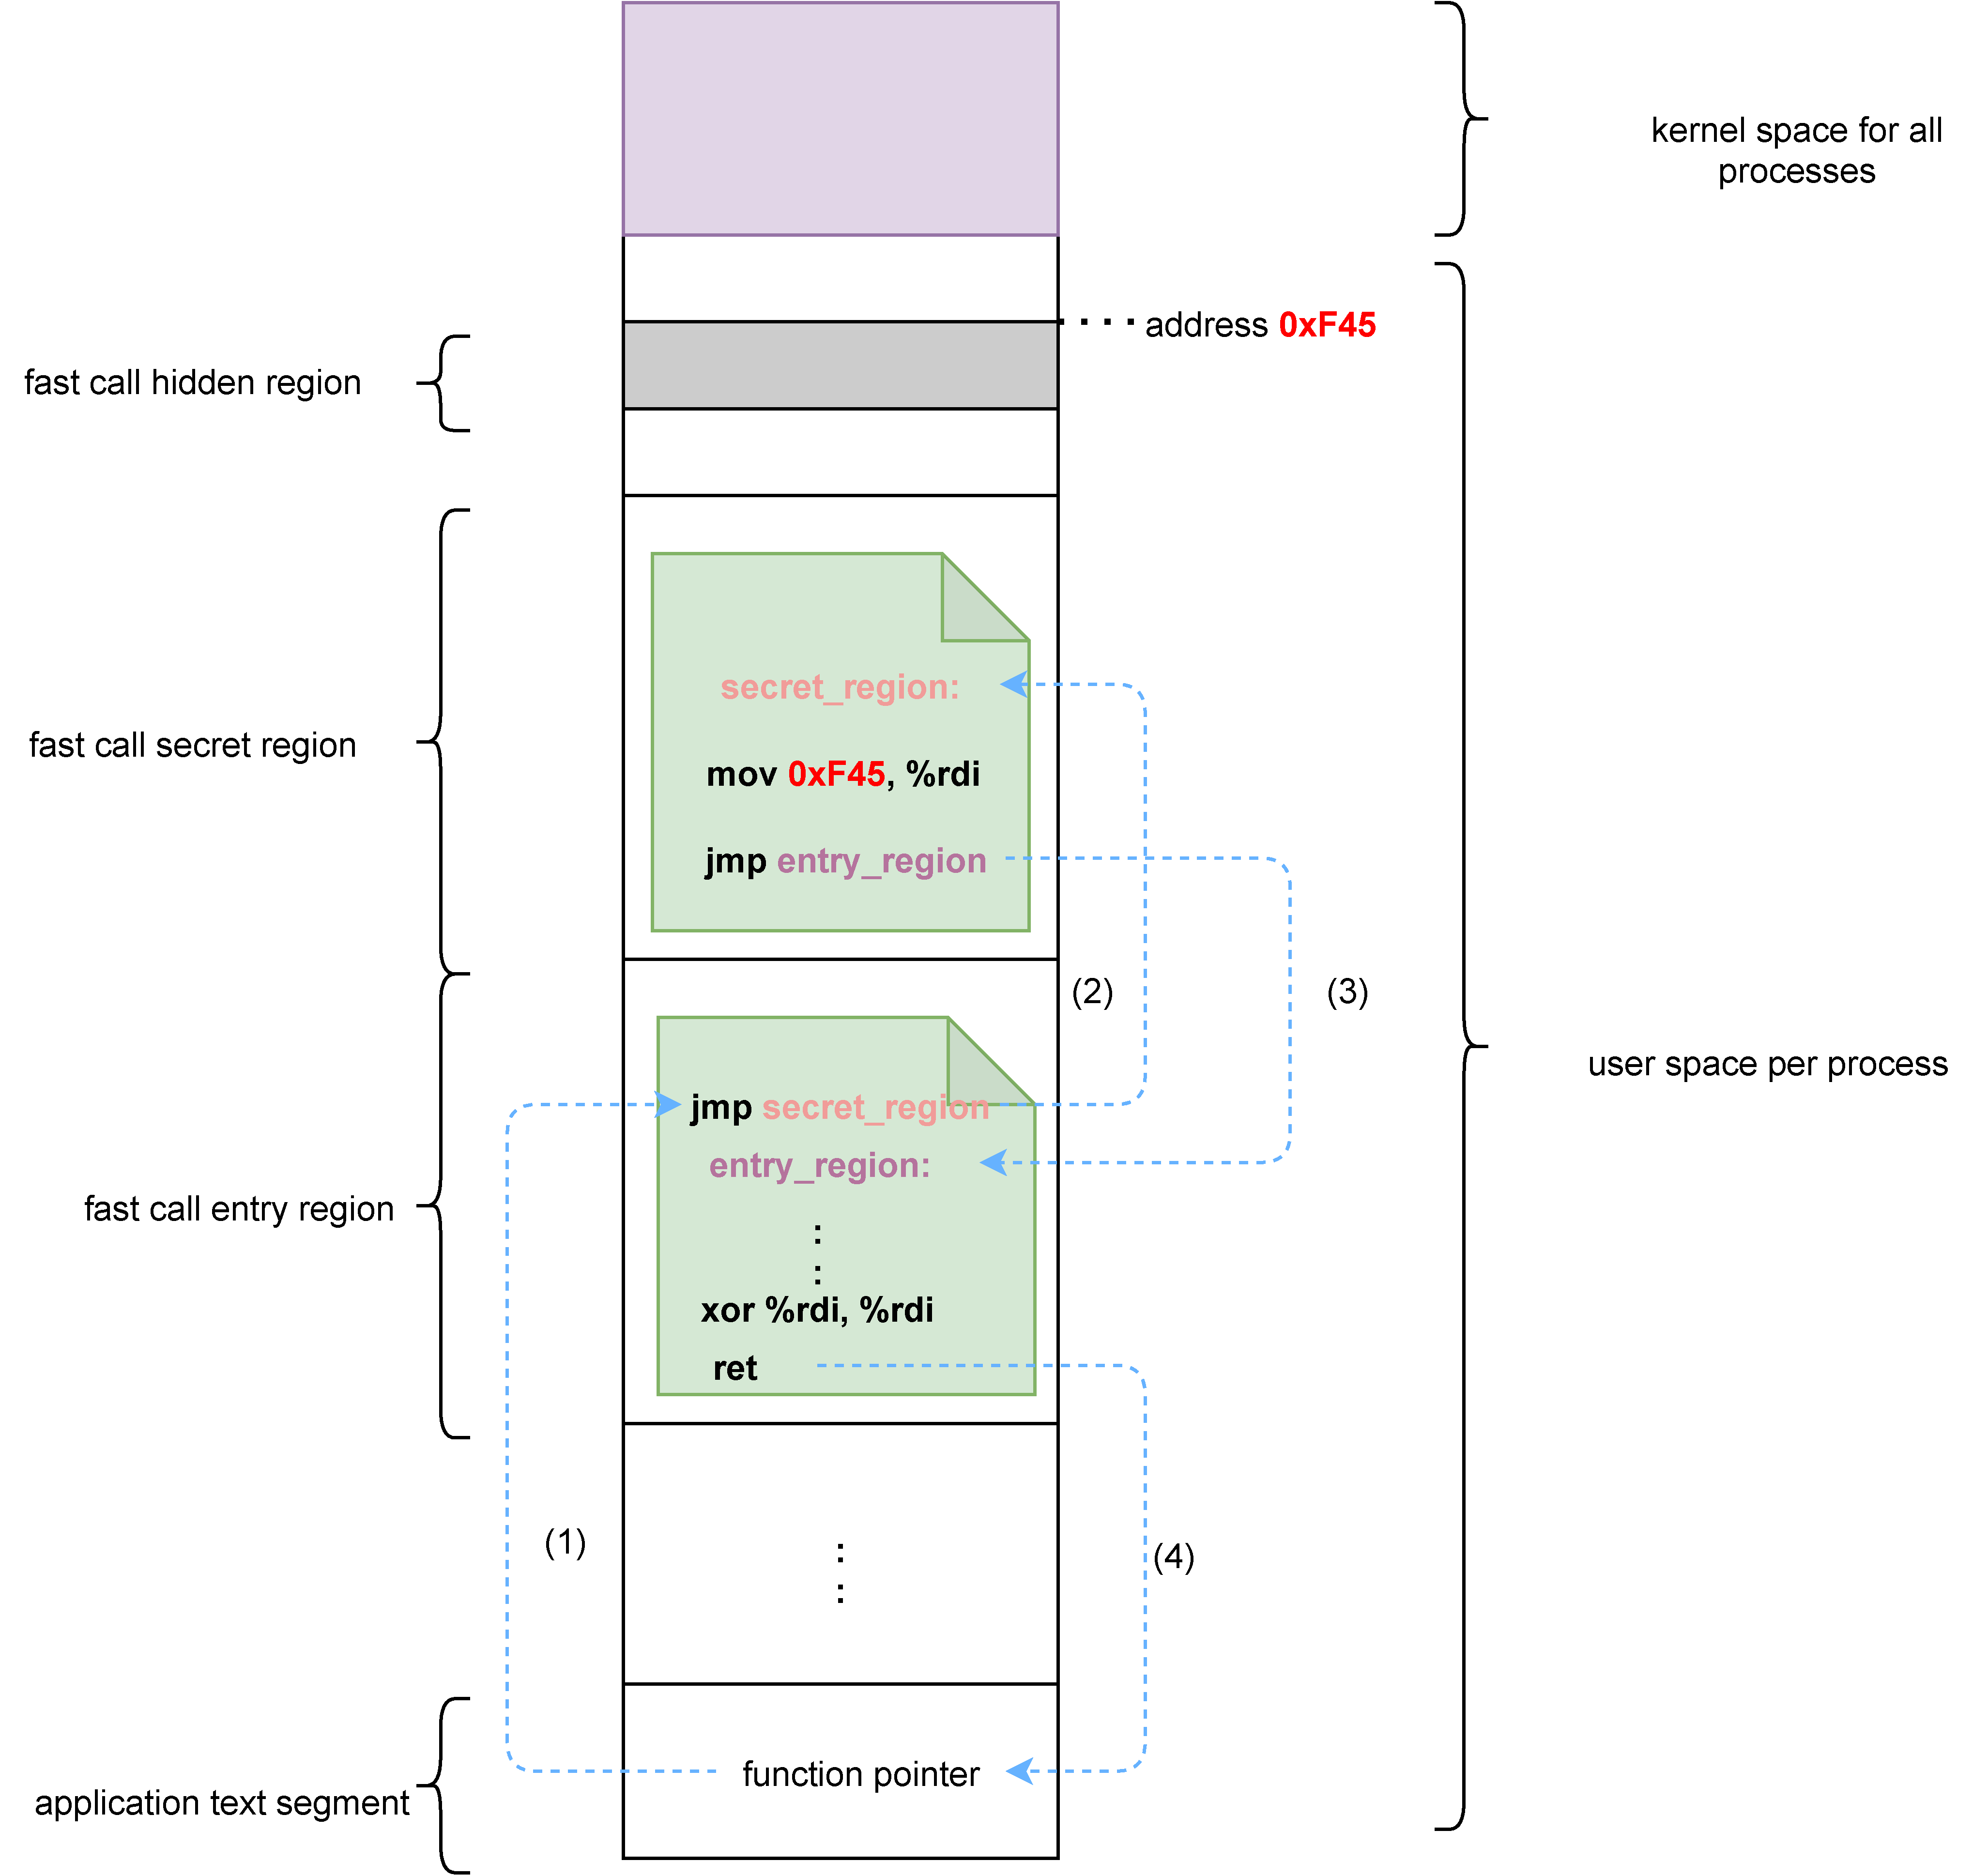
\includegraphics[width=0.8\textwidth]{images/secrt_page_3}
    \caption[Short description]{The method the fast call entry region use to retrieves a 
    secret}
     \label{fig:secrt_page_3}
  \end{figure}

  \subsection{Overwrite the value on the secret page}

  Overwriting the operands of the \emph{mov} instruction can be very tricky. 
  The fast call mechanism needs to overwrite the operand of the corresponding 
  \emph{mov} instruction on the secret page at runtime. It should be noted that 
  the fast call mechanism needs to overwrite the machine code instead of 
  assembly. The relationship between the machine code and assembly is 
  shown below. Note that machine code is architecture-dependent. Therefore, the correspondent 
  machine code of \emph{mov} instruction may be different on variant architecture.
   

  \begin{lstlisting}[style=CStyle]
    /* assembly <---> machine code */
    movq $0x7fffffffffff, %rsi  <---> 0x48 be ff ff ff ff ff  7f 00 00
  \end{lstlisting}

  In the code snippet, \emph{0x7fffffffffff} and \emph{\%rsi} represent a dummy 
  value and a register, respectively. At runtime, the fast call mechanism 
  will overwrite the dummy value in the instruction with the address of a 
  fast call hidden region. \emph{0x48 be ff ff ff ff ff  7f 00 00} represents the 
  machine code corresponding to the instruction. According to the Intel manual, 
  the bytes in the machine code have the following meanings\cite{14}:
  
  \begin{itemize}
    \item \emph{0x48} indicates that the instruction is 64-bit.
    \item \emph{0xbe} indicates that the instruction is a \emph{mov} instruction and the target register is \emph{\%rsi}.
    \item \emph{0xff ff ff ff ff 7f 00 00 } eight bytes represent the dummy value in Little Endian format
  \end{itemize}
  
  The above analysis shows that the fast call mechanism needs to pay attention to 
  the third part of the machine code, which is the dummy value in Little Endian 
  format\cite{15}. In this case, the fast call mechanism defines a \emph{char*} variable that 
  points to the instruction and increments it by 2 bytes to point to the 
  dummy value \emph{0xff ff ff ff ff 7f 00 00}. And then, the fast call mechanism cast it to a \emph{uint64\_t*}
  pointer and replace the dummy value with the address of a fast call hidden 
  region. Note here we use \emph{uint64\_t*} since the hidden region address is 64-bit.

  \begin{lstlisting}[style=CStyle]
    /* pointor to the beginning of the  mov instruction */ 
    char *poiter;
    /* skip over 0x48 and 0xbe */ 
    poiter += 2; 
    /* 
     * replace the dummy value with the address of a fast call hidden region 
     */  
    *((uint64\_t*)poiter) = 0x7ffff7fc6000; 
  \end{lstlisting}


\subsection{Jump between fast call entry and secret region}

Recall the fast call workflow. The fast call uses instruction \emph{jmp}, 
and labels to jump back and forth between the entry and the secret regions. 
Particularly, the instruction \emph{jmp label} is a relative jump\cite{14}. 
The compiler calculates the offset(distance between the instruction \emph{jmp}
and the label) at compile-time and replaces the label with the offset, i.e., 
\emph{jmp label -> jmp offset}. The relative jump then jumps to a location relative to the current 
instruction pointer at runtime, i.e., rip = rip+offset.
\begin{figure}[H]
  \centering
  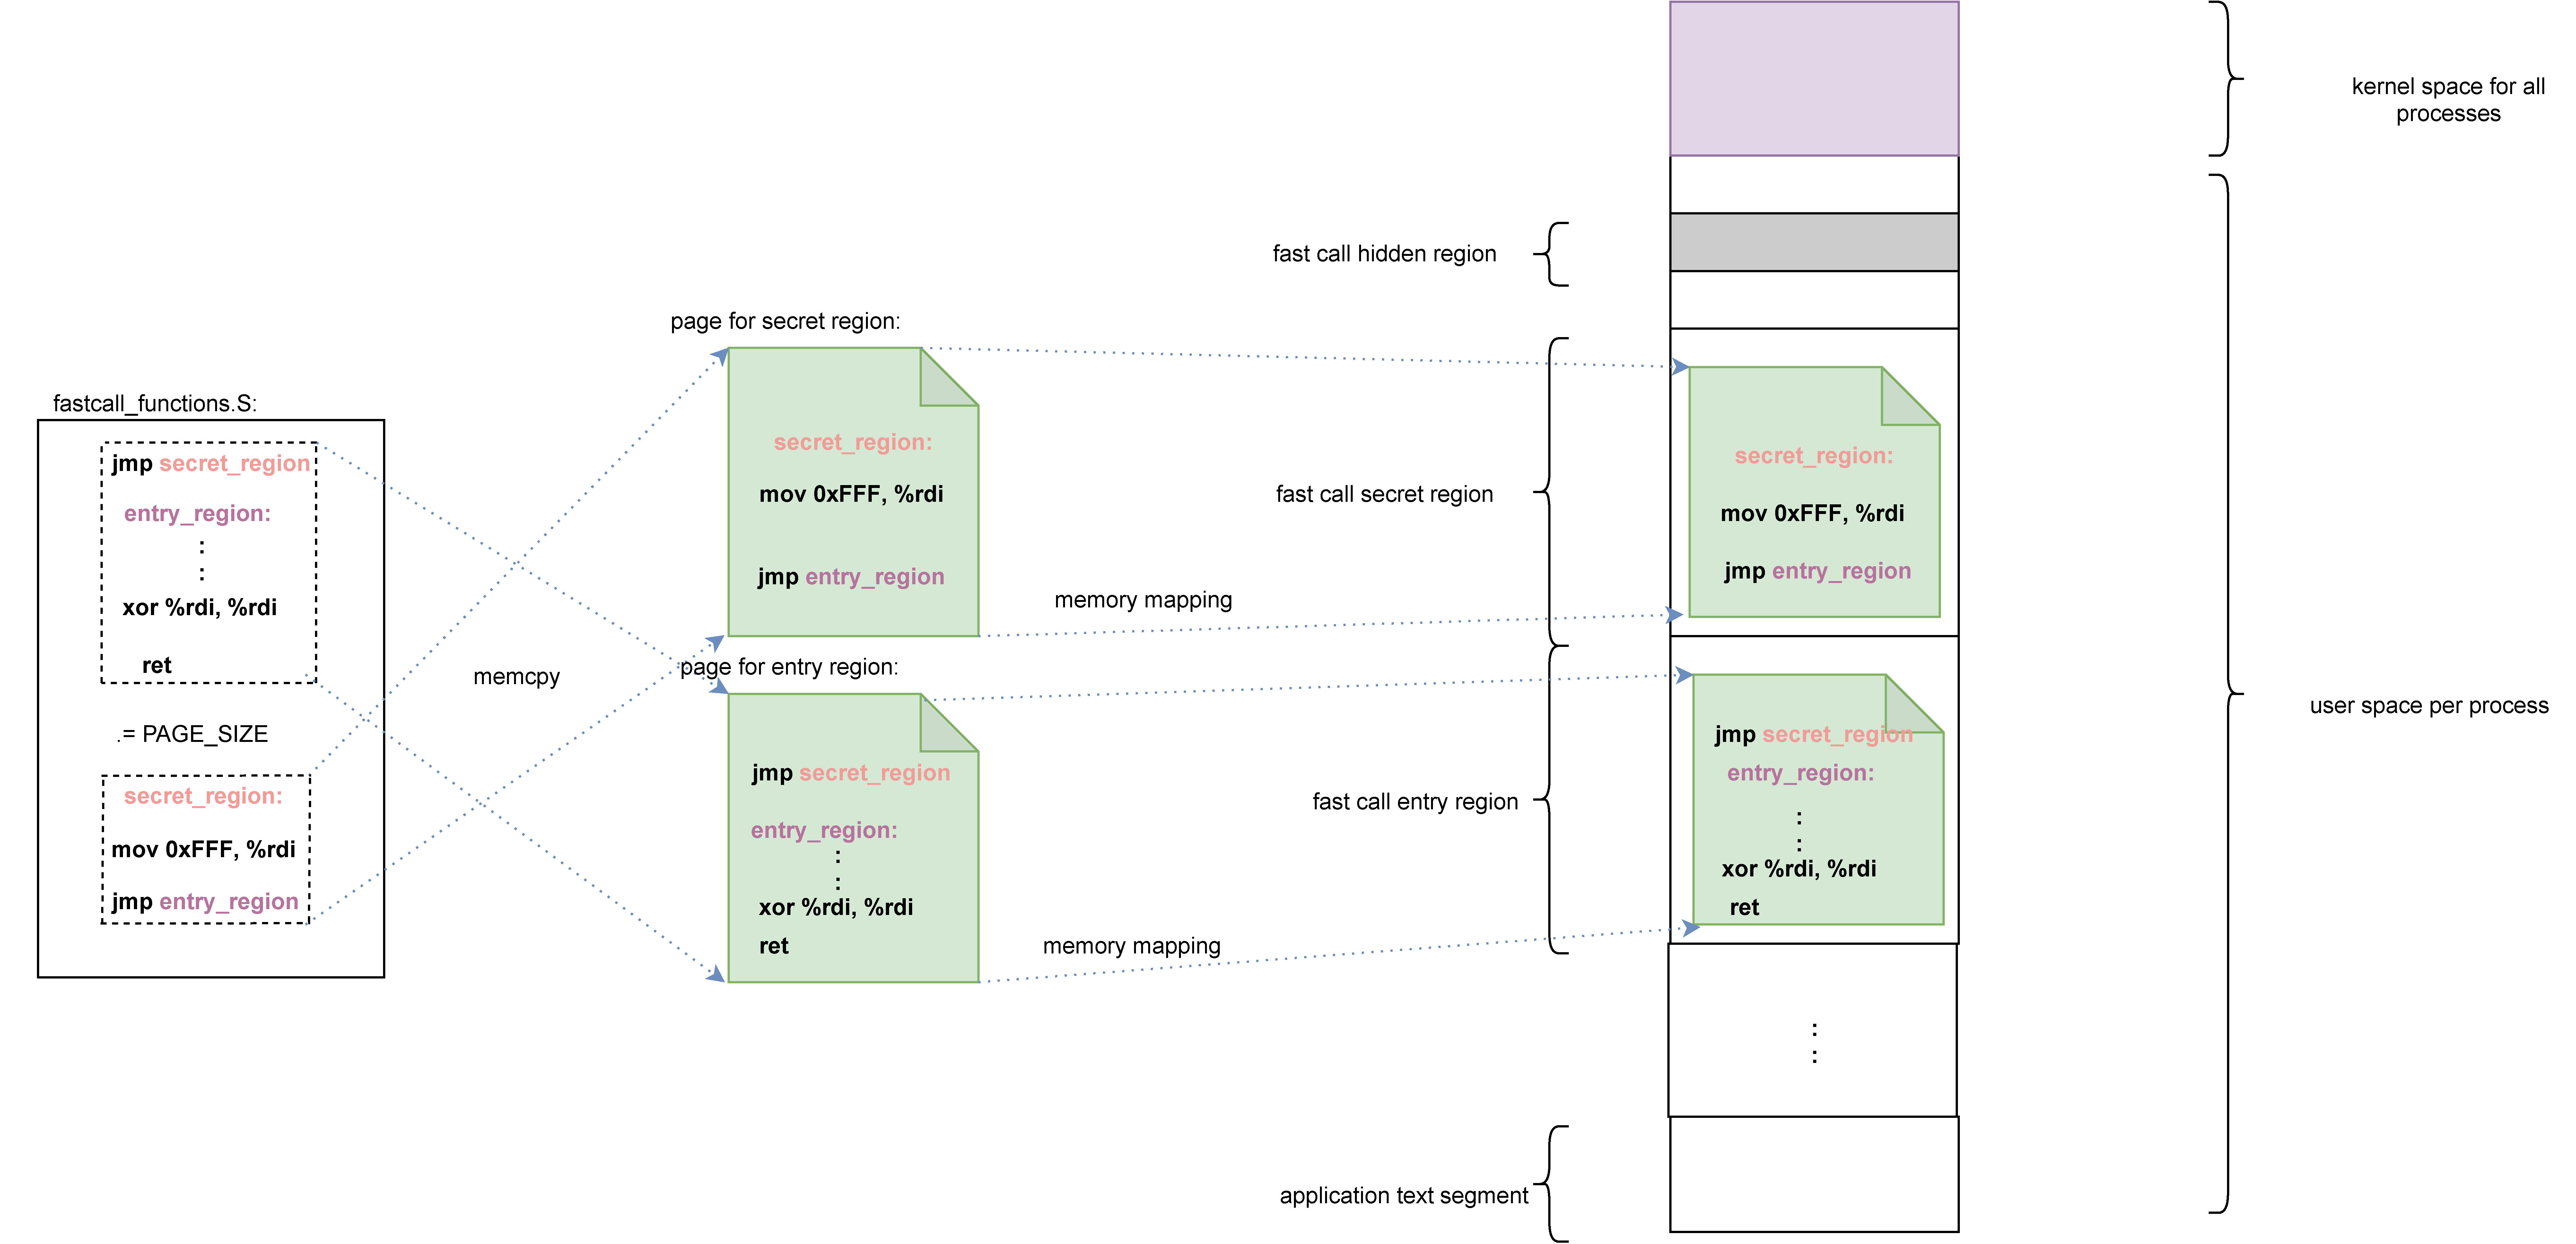
\includegraphics[width=0.8\textwidth]{images/secret_page_4}
  \caption[Short description]{The method the fast call entry region use to retrieves a 
  secret, version 2}
   \label{fig:secret_page_4}
\end{figure}
In our case, as shown in Figure \ref{fig:secret_page_4},  the fast call entry and fast call 
secret regions code are pre-written in the file \emph{fastcall\_functions}. 
The first and second code snippets represent the code for the entry and 
the secret regions, respectively. In addition,  Code snippets 1 and 2's 
distance is set to 1 page.  At compile time, the compiler replaces
\emph{entry\_region} in \emph{jmp entry\_region} and \emph{secret\_region} in \emph{jmp secret\_region}  
with appropriate offsets.  



During the fast call registration process(run time), 
the driver copies the first and second code snippets to pages for entry and secret 
regions, respectively, and passes them to the fast call infrastructure. 
The fast call infrastructure creates the entry and secret regions and maps the 
pages to those regions.  In particular, to ensure that the relative jump's offsets are valid after the pages are mapped to secret and entry regions, 
respectively, fast call mechanism needs to do two things:


\begin{itemize}
  \item Create the secret region in a 1-page size.
  \item The entry and secret regions must be adjacent, and the entry region is located above the secret region.
\end{itemize}


\section{Security issue elimination}

As we know in the Chapter \emph{Design} and the previous sections, our fast call 
mechanism is less secure than traditional methods. The reason is that fast 
calls run in user space. In this case, fast calls lose the protection of the kernel. 
Malicious users can attack fast call components in user space directly and gain the device's control.


Specifically, when the fast call entry area's code is running, a malicious 
user can obtain its secret through the \emph{GDB debugger}\cite{16}. The reason is that when 
the code in the fast call entry region is running, the secrets are stored in 
registers. An attacker can set a breakpoint at any code position in the entry
 region and observe the secrets stored in registers.

On the other hand, \emph{mprotect(2)} system call\cite{19} is a big problem. An attacker 
can leverage the system call directly to read the secret from the secret 
region since \emph{mprotect(2)} changes the secret region's access right from 
executable to readable.  Note the secret region is nothing more special 
than a virtual memory area with executable access rights. 

In addition, the \emph{proc} file system has brought us a lot of trouble. 
Each process's memory layout can be viewed by reading the file \emph{/proc/[pid]/maps} 
created by the \emph{proc} file system. Therefore,  A malicious user can find out the 
location of all hidden regions(device registers) by reading this file. This 
mechanism makes all our previous efforts to isolate applications and devices 
in vain since an attacker can bypass the fast call entry region to control 
devices directly.  

Last but not least, an attacker can set up exception handling reasonably and 
explore every address in the address space to find out the location of hidden 
regions. 

The above scenarios break the isolation between the user and the device 
provided by the fast system call mechanism and lead to security risks. 
Therefore, we need to find a way to avoid them and adequately protect 
devices from attacks. In the rest of this chapter, we will further 
explore the secret leakage that may be caused in these scenarios and 
introduce our methods to avoid such information leakage.

\subsection{\emph{GDB} scenario}
Now let's take a look at the \emph{GDB} scenario first. 
But before we start to introduce our remedies. We need to understand 
how \emph{GDB} works. \emph{GDB} stands for GNU Debugger. Developers use it extensively for error 
detection and error elimination. \emph{GDB} itself can attach to a running 
process and set breakpoints at any position in the attached process 
and observe the changes in its registers and memory at any time. 


\emph{GDB}\cite{16} are implemented through the \emph{ptrace(2)} system call. 
\emph{ptrace(2)}\cite{17} allows the parent process to config the running mode of 
the child process, set breakpoints in the child process, observe or 
change the value of the child process's registers, and track the system 
call of the child process.

\begin{figure}[tbp]
  \centering
  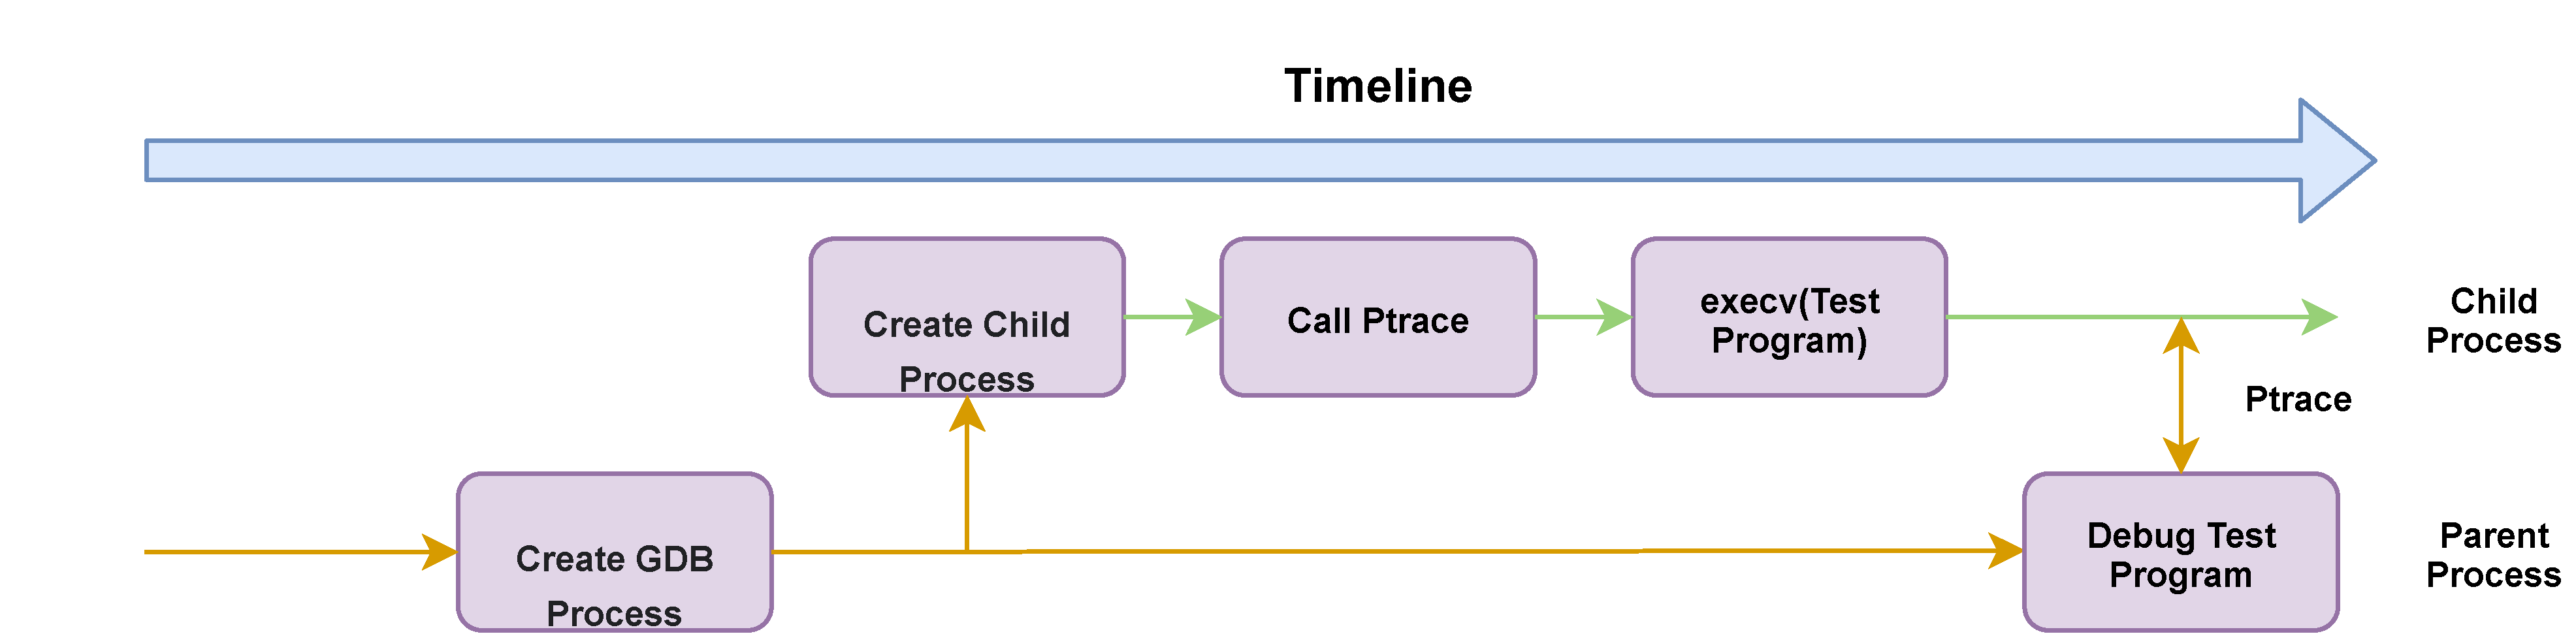
\includegraphics[width=0.8\textwidth]{images/GDB_METHOD1}
  \caption[Short description]{First GDB workflow}
  \label{fig:GDB_METHOD1}
\end{figure}

In general, there are two working modes in \emph{GDB}. Figure \ref{fig:GDB_METHOD1} shows 
the \emph{GDB}'s first workflow. A process starts running the \emph{GDB} program, 
and then \emph{GDB} creates a child process through the \emph{fork} system call. 
The child process needs to do two things. First, the child 
invokes the \emph{ptrace(2)} system call to attaches its parent to itself. 
Then the child executes the test program through the \emph{exec(3)} 
system call. Note that the \emph{GDB} process is the \emph{tracer} and its child 
is the \emph{tracee}. After the above work is completed, the tracer can debug \emph{tracee} 
through the \emph{ptrace(2)} system call.



\begin{figure}[tbp]
  \centering
  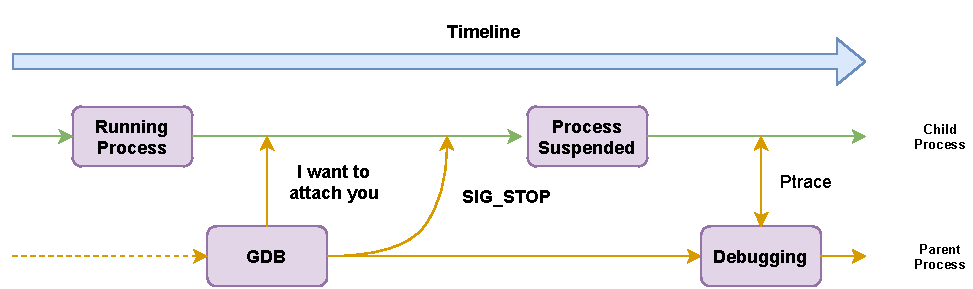
\includegraphics[width=0.8\textwidth]{images/GDB_METHOD2}
  \caption[Short description]{Second GDB workflow}
  \label{fig:GDB_METHOD2}
\end{figure}

\emph{GDB} can also debug the running process. As shown in Figure \ref{fig:GDB_METHOD2}, 
the \emph{GDB} process can turn the running process into its child process, 
attach itself to the child, and send \emph{SIGSTOP} to the child. 
The child stops running after receiving the \emph{SIGSTOP} signal, 
indicating that it is ready to be debugged.

All in all, for the \emph{tracee}, whether it is a running process or 
a new process, \emph{GDB} will turn the \emph{tracee} into its child process 
through the \emph{ptrace(2)} system call. Afterward, the \emph{GDB} can view and modify 
the \emph{tracee}'s memory, stack, and registers.

As we mentioned before, the entry region retrieves secrets 
from the secret region through registers and keeps them in registers until the fast call is completed. 
Therefore, An attacker can exploit \emph{GDB}  to obtain the secrets 
and gain control of a device.  Note that \emph{GDB} is only an example of obtaining 
secrets based on \emph{ptrace(2)}. Any attacker can imitate the two working modes of 
\emph{GDB} and use \emph{ptrace(2)} to obtain secrets from entry region as fast call is running.

In general, it is hard to avoid a process that is about to register 
fast calls from being tracked through \emph{ptrace(2)}.  For instance, 
in the first \emph{GDB}  working model, the child first calls \emph{ptrace(2)} to 
attach itself to its parent then execute the test file registering for fast calls. 
In this case, we can't let the \emph{ptrace(2)} in-kernel handler routine reject the child's 
request since the routine does not know that the child is going to execute the test file 
registering for fast calls. On the other hand, once the child has been traced and executed 
the test file, the child can not detach itself in the fast call infrastructure because 
\emph{ptrace} does not allow \emph{tracee} to be detached by itself.

Our goal is to prevent the \emph{tracer} from reading the 
\emph{tracee}'s registers when \emph{tracee} has registered fast calls. 
Since the \emph{tracer} exploits \emph{ptrace(2)} to reads \emph{tracee}'s registers, 
we can let the \emph{ptrace(2)} handler function check whether \emph{tracee} has 
registered fast calls before returning the data in \emph{tracee}'s registers.
Specifically, we add a new variable \emph{fastcall\_registered} 
in the process address space descriptor \emph{mm\_struct(2)}\cite{10.5555/983550} to mark whether a process
address space has fast calls. When the tracer calls \emph{ptrace(2)} system call 
to view the \emph{tracee}'s register, \emph{ptrace(2)} handler function in kernel can judge whether
\emph{tracee} has registered fast calls by checking \emph{fastcall\_registered} in 
the \emph{tracee}'s address space descriptor. If \emph{tracee} has already 
registered fast calls, \emph{ptrace(2)} system call handler function should 
directly return the error \emph{EPERM} to the tracer, indicating that this 
operation is not permitted.

The variable \emph{fastcall\_registered} is managed by fast call 
infrastructure. During the fast call registration process,  
the fast call infrastructure sets \emph{fastcall\_registered} in the current 
\emph{mm\_struct} to true. On the other hand, at the end of the fast call 
deregistration process, the fast call infrastructure checks whether 
the current address space still has fast calls. It set \emph{fastcall\_registered}  
to false if the current address space does not have fast calls anymore.


It should be noted that when a process is created, we initialize 
the \emph{mm\_struct}'s member \emph{fastcall\_registered}  to false because 
the fast call mechanism prohibits two processes from sharing fast calls.
 In other words, when process A uses \emph{fork()}\cite{18} to create a child process B, 
 B will not copy the virtual memory areas\cite{10.5555/983550}  belonging to fast calls in A, 
 which means that B has not registered any fast calls. 
 Therefore, we should set \emph{fastcall\_registered}  in B's address space 
 descriptor to false when B initializes its address space descriptor.

 The advantage of having variable \emph{fastcall\_registered} in the address space 
 descriptor is obvious.  We have avoided secrets leakage from \emph{ptrace} under 
 multithreading. All operations of \emph{ptrace}, including attachment and detachment, 
 are per thread. Note that threads and processes are represented by \emph{task\_struct}
 in the kernel, and the only difference between them is that threads share 
the same address space descriptor. Therefore, we add \emph{fastcall\_registered} 
in the address space descriptor to prevent secrets leakage from any thread 
been traced if its address space has fast calls.


\subsection{mprotect}
As we mentioned earlier, an application can call \emph{mprotect(2)}  
system call\cite{19} to change the address space's access protection, 
e.g., changing the access right of a particular area in the address 
space from executable to readable.  A malicious user can leverage the 
\emph{mprotect(2)} to change the access right of a fast call's memory areas to 
damage the fast call. Specifically, an attacker can change the fast 
call entry region's access right from readable to writable so that the attacker can overwrite 
the code mapped on this region to change the fast call's behavior. 
Another attack path is that the attacker directly changes the secret 
region's access right from executable only to readable. In this way, 
the attacker can read the secrets on the secret region and bypass the 
fast call to manipulate a device.
\begin{figure}[H]
  \centering
  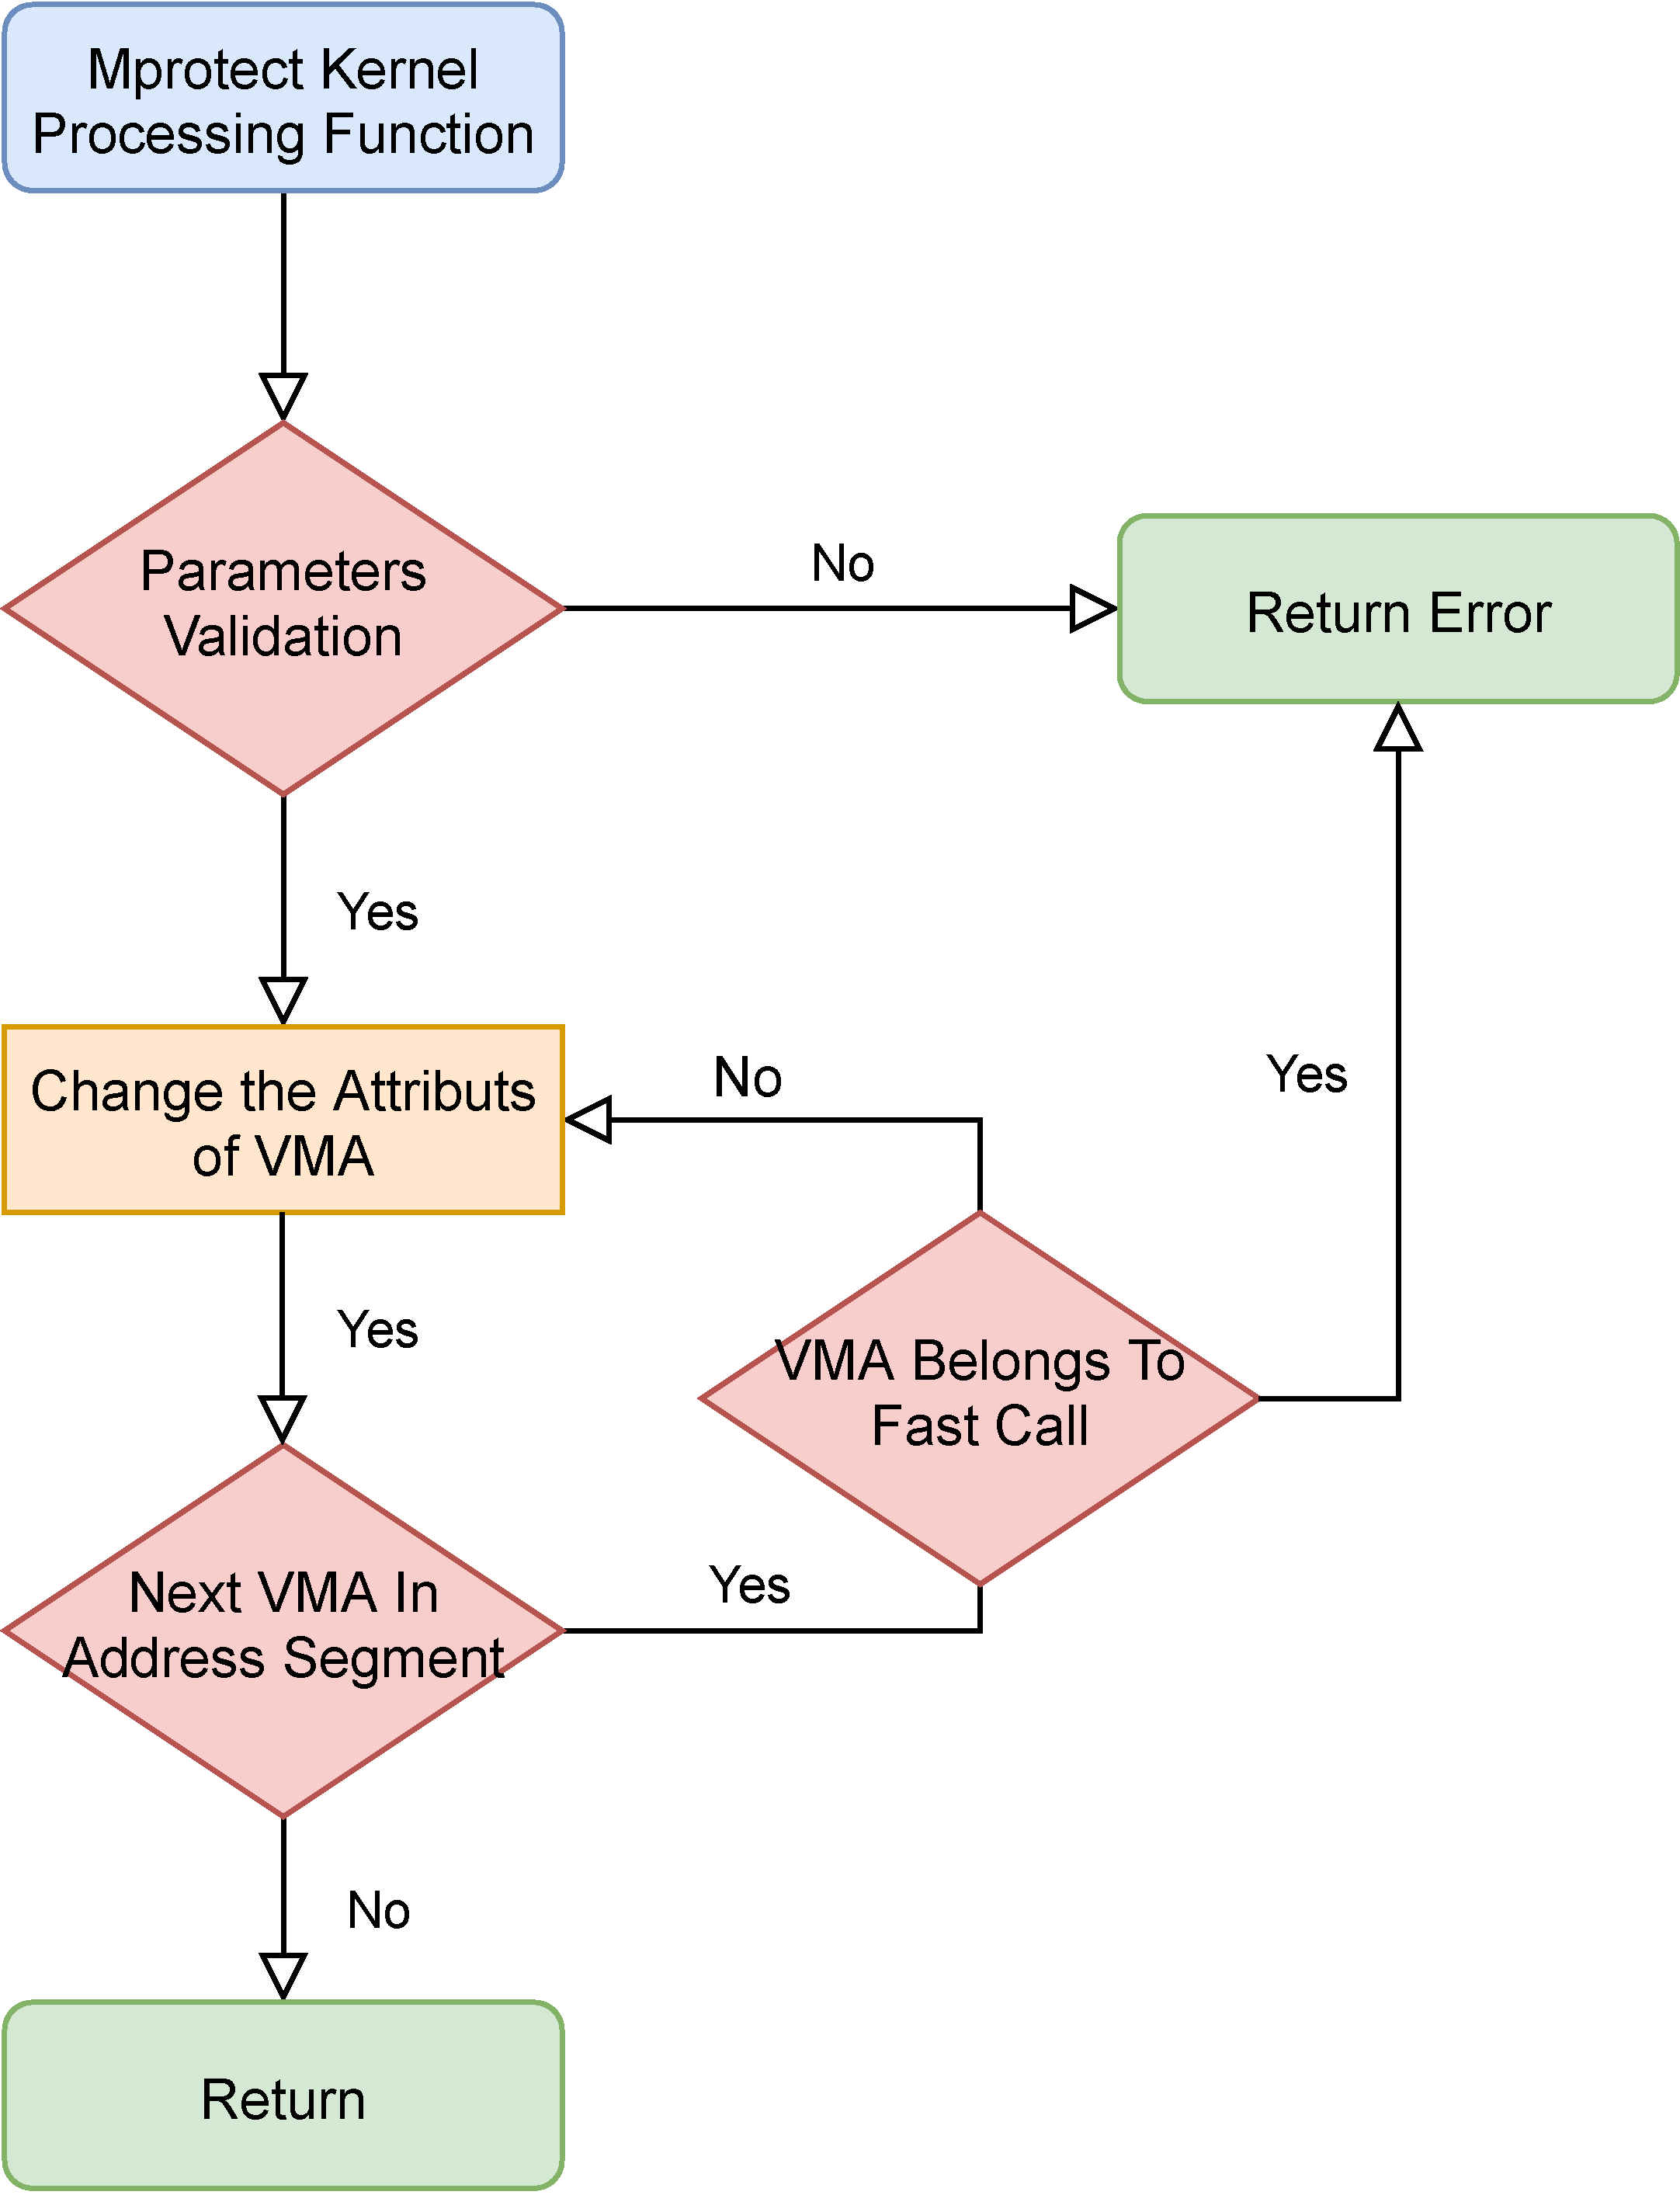
\includegraphics[width=0.8\textwidth]{images/MPROTECT}
  \caption[Short description]{MPROTECT workflow}
  \label{fig:MPROTECT}
\end{figure}

Figure \ref{fig:GDB_METHOD1} shows how fast call mechanisms avoid \emph{mprotect(2)} 
changing the access right of fast calls'virtual memory areas. 
Note that the process address space\cite{10.5555/983550} is composed of virtual memory areas\cite{10.5555/983550}.  
When \emph{mprotect(2)} system call is called to change the access rights on a 
consecutive address range in the process address space, the \emph{mprotect(2)} 
handler routine in the kernel validates the incoming parameters. 
If the request from user space is legal, the routine 
traverse all \emph{VMAs} in the address segment specified in the parameters
 and change the access right of each \emph{VMA}. Therefore, while the function 
 traverses all the \emph{VMAs} in the address segment, we could add the following 
 code to check whether a \emph{VMA} belongs to fast calls that the current process 
 has registered. If the \emph{VMA} belongs to a fast call, the routine 
 should terminate and return an error before changing the \emph{VMA}'s access right.

\begin{lstlisting}[style=CStyle]
  if (VMA_is_special_mapping(VMA, &fastcall_pages_mapping))
    goto out;
\end{lstlisting}
 

\subsection{Prevent attacker from exploring the address space}
Now we have to face the direct attack on the hidden region. 
The hidden region represents the device registers mapped to the
 process address space\cite{10.5555/983550} in a fast call. The fast call entry region 
 can obtain the address of a  hidden region from the secret region and
  control the device to complete specific operations. Because the 
  registers are directly mapped to the user space, all operations 
  on the registers are as fast as ordinary memory access. However, 
  this also brings considerable problems. A malicious process can 
  leverage the fast call mechanism to map registers of a device 
  they want to control to their address space and then explore the 
  entire address space to find the location of the registers. 
  In other words, a malicious process can reasonably set its 
  action on the segmentation fault\cite{21} and explore the entire address space to find the hidden region.

Generally speaking, the segmentation fault is caused by two reasons. 
The first reason is that a process has accessed an address 
that it does not have permission to access, and the other 
reason is that a process has accessed an address that the 
kernel has not allocated. We are more interested in the 
second case in this section. In this case, the kernel sends 
\emph{SIGSEGV}\cite{21} signal to the process. By default,  the process will 
terminate when it receives \emph{SIGSEGV}.  However, a process can 
change its action on a signal through \emph{sigaction(2)}\cite{20}. This 
means that a process has the ability to ignore \emph{SIGSEGV} 
and continue to run. Another possibility is that a process 
can use \emph{mmap(2)}\cite{22} to allocate memory for all unallocated 
areas in its address space. In this way, when the attacker 
explores the entire memory space, segfault will not occur at all.

\begin{figure}[H]
  \centering
  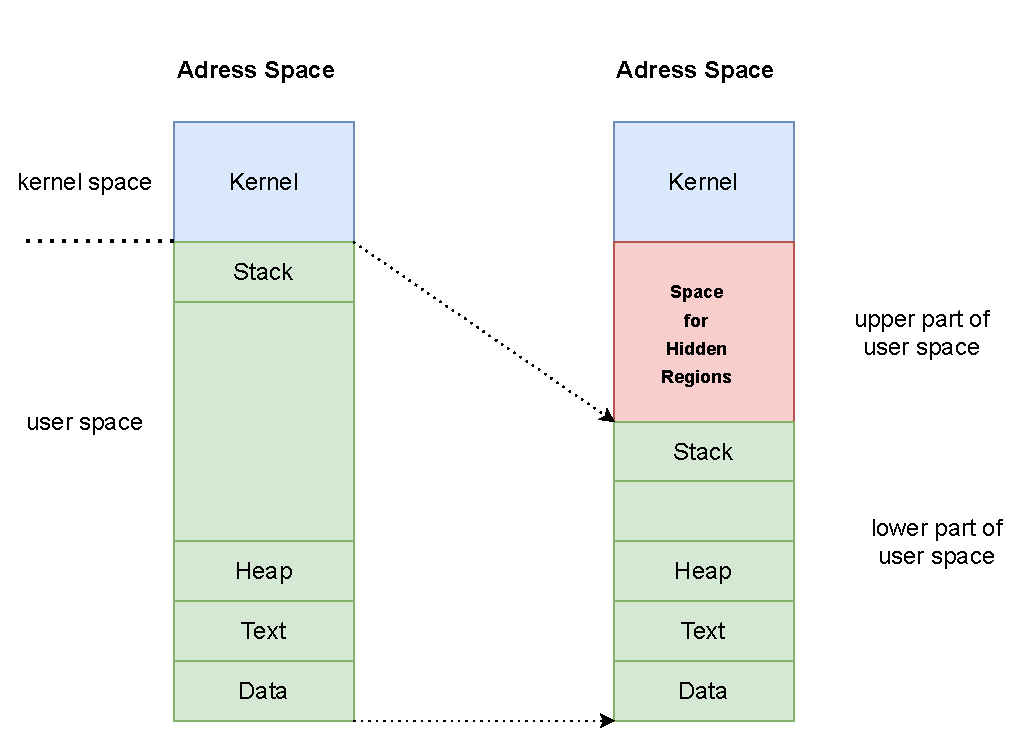
\includegraphics[width=0.8\textwidth]{images/Seperateuserspace}
  \caption[Short description]{Prevent attacker from explore the address space}
  \label{fig:Seperateuserspace}
\end{figure}


The fast call mechanism must avoid an attacker from exploring 
the address space in those two ways. Figure \ref{fig:Seperateuserspace} 
shows the method that the fast call mechanism uses to address this issue. 
After the fast call mechanism is enabled, each user space is divided into
two parts. The lower part is used as the original address space to 
allocate such as stacks, program code segments, etc., while the upper 
part is dedicated to allocating all fast calls' hidden regions. 
In particular, we prohibit any request to allocate memory in the 
upper half of the address space except requests from the in-kernel 
fast call infrastructure. In other words, a process cannot call \emph{mmap(2)} 
to allocate memory in the upper half of its address space.

In addition, we have changed the signal that the kernel 
sends to the process when the segmentation fault occurs 
in the upper half of the address space. Specifically, 
when a process accesses an unallocated memory address 
in the upper half of the address space, the kernel page 
fault handler will send \emph{SIGKILL}\cite{21} to the process instead 
of \emph{SIGSEGV}. The advantage of \emph{SIGKILL} is that the process 
cannot change its action when receiving the signal, which means 
that the process has no choice but to kill itself 
when it receives this signal.

To sum up, the fast call mechanism divides the address space 
into two parts so that the hidden regions have exclusive space,
which significantly reduces the attack risk. Because, in this 
case, a malicious user has only one chance to determine the 
location of hidden regions.  If a malicious user accesses a 
memory address that has not been allocated in the upper part
of the user space, the kernel will send a \emph{SIGKILL} to kill 
the malicious user. Thus, an attacker can no longer find hidden 
regions by exploring the entire address space.


\subsection{Prevent attacker from viewing the address space layout}

After understanding how the fast call mechanism solves the possible attacks 
against different components in the fast call, let us finally look at the security 
vulnerability that has the most severe impact on the fast call and is also the most 
easily exploited by malicious users. That is the virtual file\emph{/proc/pid/maps}\cite{23}. 

The virtual file \emph{/proc/pid/maps} stands for a file that contains the address 
space layout of the process \emph{pid}. It is a virtual file because the kernel generates 
files dynamically. This means that if the address space layout changes, the contents 
of the file will change too. The following code snippet shows the output of the 
command  \emph{cat /proc/pid/maps} in the shell. That is the process \emph{pid’s} address space layout. 
From the kernel’s perspective, each row in the figure stands for a virtual memory area(VMA). 
In addition, the kernel manages all \emph{VAMs}\cite{10.5555/983550} in a process through a \emph{VMAs list}. As mentioned above, 
the three components in a fast call, the entry, secret and hidden region, are just three 
virtual memory areas in the process address space. Therefore, when a process has registered 
for fast calls, the kernel adds the \emph{VAMs} created for the fast call to the \emph{VAMs list}. 
Later, the kernel generates the virtual file \emph{/proc/pid/maps} according to the VMA in the 
\emph{VAMs} list if someone opens it. In this case, the file contains the information about 
the fast call's three components, e.g. the start and end address of the fast call hidden region. 

 
\begin{lstlisting}[style=BASHStyle]
  #!/bin/bash
  #!sudo cat /proc/1/maps
  7fd9b1f77000-7fd9b1f78000 r--p            /usr/lib/x86_64-linux-gnu/ld-2.31.so
  7fd9b1f78000-7fd9b1f79000 rw-p            /usr/lib/x86_64-linux-gnu/ld-2.31.so
  7fd9b1f79000-7fd9b1f7a000 rw-p  
  7ffe334f0000-7ffe33511000 rw-p            [stack]
  7ffe33594000-7ffe33598000 r--p            [vvar]
  7ffe33598000-7ffe3359a000 r-xp            [vdso]
  ffffffffff600000-ffffffffff601000 --xp    [vsyscall]
\end{lstlisting}

This file is highly harmful to the fast call mechanism since 
it leaks all information about the fast calls that the fast call 
mechanism tries to hide. Therefore, we must avoid the kernel from 
including information about fast calls when generating this file. 
Before explaining how the fast call mechanism solves this security 
vulnerability, let us first look at how this file is generated.

The file\emph{/proc/pid/maps} is a virtual file dynamically
generated by the process information pseudo-filesystem\cite{23}(\emph{PROC}). 
Specifically, \emph{PROC} automatically generates the file according to 
the process address space's memory layout when a user opens the file. 
Therefore, when the memory layout of the process changes, the content 
of the file changes as well. In the kernel, the file supports four operations, 
namely, opening the file (\emph{open}), reading the content of the file (\emph{read}), 
changing the starting position of reading the file (\emph{llseek}), and 
closing the file (\emph{release}).  Internally, these four operations 
encapsulate a sequence file\cite{24} and call the corresponding function in the sequence file.
The sequence file completes \emph{VAM's} traversal in the process address space 
through the \emph{VMA list}. For example, the open operation 
creates a sequence file in the kernel, and the read operation uses the 
functions provided by the sequence file to traversal the \emph{VAMs list} and copies 
each \emph{VAM}'s information to user space, etc.





\begin{figure}[tbp]
  \centering
  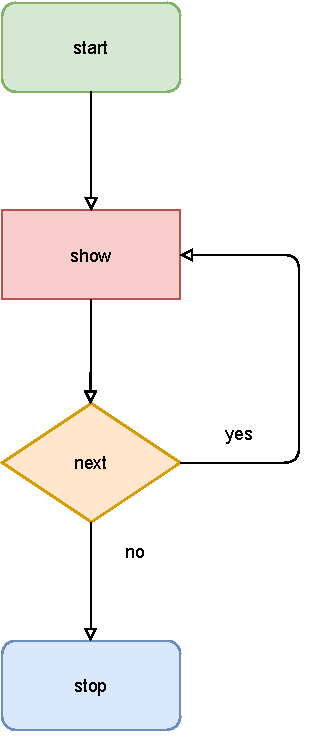
\includegraphics[width=6cm,height=9cm]{images/sequence_file}
  \caption[Short description]{Sequence file workflow}
  \label{fig:sequence_file}
\end{figure}

The sequence file is an iterator provided by \emph{PROC}, 
which is specially used to traverse the kernel data structure 
such as a list to generate virtual files. As shown in Figure \ref{fig:sequence_file}, this 
iterator consists of four methods, namely start(), next(), stop() 
and show(). Its working principle is very similar to the iterator in C++. 
In our case, the start() function will be used to initialize the iterator 
that traverses the \emph{VAM} list. The next() function will move the iterator 
forward to the next \emph{VAM} in the list. The show() function is similar 
to the dereference operator in C++. In this function,  the iterator is 
dereferenced to obtain the \emph{VAM} pointed by the iterator, then the 
information about the \emph{VAM} is written into a buffer whose contents 
will be copied to the user space later. If the traversal is complete, 
stop() is called to destroy the iterator.

Therefore, the idea about preventing information leaks is the
same as what we did in \emph{mprotect(2)}. We add the following code in show() to 
check whether a \emph{VAM} belongs to fast calls.  If the \emph{VAM} 
belongs to fast calls, the show function should skip the \emph{VAM} 
instead of adding information about this \emph{VAM} to the buffer. 
In this way, the file does not show any information about 
fast calls' components anymore.



\begin{lstlisting}[style=CStyle]
  if (VMA_is_special_mapping(VMA, &fastcall_pages_mapping))
    goto out;
\end{lstlisting}


\cleardoublepage



%%% Local Variables:
%%% TeX-master: "diplom"
%%% End:


